\documentclass[11pt,fleqn,twoside]{book} % Default font size and left-justified equations

\newcommand{\booknameSimple}{PyAIML Notes V3}
\newcommand{\authornameSimple}{Rohnak Agarwal}

\newcommand{\bookname}{\href{https://www.overleaf.com/read/kxpnmgkydymz\#606c1d}{\booknameSimple}}
\newcommand{\authorname}{\href{mailto:rrka79wal@gmail.com}{\authornameSimple}}

\usepackage{fontawesome5}


\RequirePackage[hyphens]{url} 
% This package allows proper handling of URLs in the document, ensuring they are properly hyphenated if they span multiple lines.

\usepackage{amssymb} % for symbols like checkmark

\usepackage[top=2cm,bottom=2cm,left=2.2cm,right=2.2cm,headsep=10pt,a4paper]{geometry} 
% Configures the page layout with specified margins and paper size (A4), including top, bottom, left, and right margins, and the header separation.

\usepackage[dvipsnames,table]{xcolor} 
% Provides color support in the document, allowing named colors and coloring of tables and other elements.

\usepackage{mathptmx} 
% Changes the default text font to Adobe Times Roman and the math font to the Symbol, Chancery, and Computer Modern fonts for mathematical symbols.

\usepackage{mathrsfs} 
% Loads the mathrsfs package to provide a script-like math font (commonly used for calligraphic letters in mathematics).

\DeclareMathAlphabet{\mathcal}{OMS}{cmsy}{m}{n} 
% Redefines the \mathcal font to make it less curvy and more suited for mathematical characters.

\usepackage[utf8]{inputenc} 
% Specifies the input encoding of the document as UTF-8, enabling support for special characters and accented letters.

\usepackage[T1]{fontenc} 
% Ensures the use of an 8-bit font encoding that provides access to 256 glyphs, improving the document's character handling, especially for European languages.

\usepackage{amsmath} 
% Provides advanced mathematical features, including various environments and tools for handling mathematical equations and symbols.

\everymath{\displaystyle}   
% Ensures that inline math expressions are displayed in "display style," which is usually used for equations to make them larger and more readable.

\everydisplay{\displaystyle} 
% Ensures that display math (e.g., equations shown on their own line) uses the "display style" for larger symbols and better readability.

\setcounter{MaxMatrixCols}{20} 
% Increases the maximum number of columns allowed in a matrix to 20 (the default is 10), useful for large matrices in math environments.

\usepackage{mathtools} 
% Extends the functionality of the amsmath package, adding additional tools and enhancements for working with mathematical expressions.

\usepackage{float} 
% Allows better control over the placement of figures and tables, particularly with the "H" option that forces figures to appear exactly where they are in the code.

\usepackage{longtable} 
% Provides support for tables that span multiple pages, useful for large tables that need to be split across different pages.

\usepackage{tabularx}


\usepackage{multicol,multirow} 
% The multicol package allows creating multi-column text layouts, and multirow enables the merging of rows in tables.

\usepackage{graphicx} 
% Required for including graphics (images) in your document, allowing for resizing, rotation, and positioning.

\usepackage{enumitem} 
% Enhances the customization of lists (enumerated and itemized), providing control over label format, spacing, and more.
\setlist{itemsep=0.1cm, topsep=0.1cm}


\usepackage[none]{hyphenat} 
% Disables hyphenation in the document, preventing words from being broken at the end of lines.

\usepackage{bbm} 
% Provides blackboard bold math symbols (e.g., \mathbb{N} for natural numbers) used in mathematics.

\usepackage{bm} 
% Provides support for bolding mathematical symbols and expressions (e.g., \bm{a} for bold vector a).

\usepackage{nameref} 
% Allows for referencing sections, equations, figures, and tables by their names instead of numbers.

\usepackage{datetime} 
% Provides tools for working with dates and times in LaTeX, such as displaying the current date in different formats.

\usepackage{cancel} 
% Adds the ability to "cancel" or strike out parts of mathematical expressions (e.g., crossing out terms).

\usepackage{scrextend} 
% Provides additional functionality for document layout and formatting, such as custom margins and page styles.

% Import the pifont package to use special symbols like checkmarks and crosses
\usepackage{pifont}% http://ctan.org/pkg/pifont

% Define a custom command \xmark to represent a cross mark using the 'ding' symbol (code 55)
\newcommand{\xmark}{\ding{55}}

\usepackage{lipsum} % Inserts dummy text


\usepackage{wrapfig}





\usepackage[style=numeric,sortcites=true,autopunct=true,autolang=hyphen,hyperref=true,abbreviate=false,backref=false,backend=biber]{biblatex}
% The `biblatex` package is used for creating and formatting bibliographies. The options here configure how the bibliography is displayed:
% - `style=numeric`: Uses a numeric citation style (e.g., [1], [2], etc.).
% - `sortcites=true`: Sorts the citations in the order they are referenced.
% - `autopunct=true`: Automatically adds punctuation marks after citations where necessary.
% - `autolang=hyphen`: Ensures correct hyphenation rules based on the language setting.
% - `hyperref=true`: Enables hyperlinks in the bibliography and citation links.
% - `abbreviate=false`: Avoids abbreviation of publisher names.
% - `backref=false`: Disables back references, where the bibliography shows which pages a citation appears on.
% - `backend=biber`: Specifies the backend for processing the bibliography, using `biber` as the citation manager.


\addbibresource{bibliography.bib} 
% Specifies the `.bib` file (bibliography file) containing the references to be used in the document. Here, it's named `bibliography.bib`.

\DeclareSortingTemplate{sort-tmpl}{
    \sort{
        \field{type}
    }
    \sort{
        \field{title}
    }
    \sort{
        \field{year}
    }
}

% This custom sorting scheme defines how references should be sorted in the bibliography. It sorts first by title, then by year, and finally by author.

\ExecuteBibliographyOptions{sorting=sort-tmpl} 
% Applies the sorting scheme defined earlier, sorting the bibliography entries based on the `title` field.

% remove full stop at end of bib entry
\renewcommand{\finentrypunct}{}


\DeclareBibliographyDriver{book}{% 
  \usebibmacro{bibindex}%
  \usebibmacro{begentry}%
  \iffieldundef{type}{}{%
    \textsc{\printfield{type}}:
  }
  \normalfont
  \thefield{title}%
  \iffieldundef{series}{}{
    \ \textsc{Series}: \printfield{series}
  }
  \ \textsc{Author(s)}: \printnames{author}%
  \iflistundef{publisher}{}{
    \ \textsc{Publisher}: \printlist{publisher}
  }
  \iffieldundef{year}{}{
    \ \textsc{Year}: \printfield{year}
  }
  % \\\textsc{Publisher \& Year}: \printlist{publisher},%
  % \ \printfield{year}%
  \iffieldundef{url}{}{%
    \\ \textsc{url}: \url{\thefield{url}}
  }%
  \usebibmacro{finentry}%
} 


\DeclareBibliographyDriver{online}{% 
    \usebibmacro{bibindex}%
    \usebibmacro{begentry}%
    \iffieldundef{type}{}{%
        \textsc{\printfield{type}}:
      }
    \normalfont\thefield{title}%
    \iffieldundef{url}{}{%
        \\ \textsc{url}: \url{\thefield{url}}
    }%
    \usebibmacro{finentry}%
} 







\usepackage{array} 
% Provides additional tools for defining and customizing tables. It allows for more control over column formatting, alignment, and other table features.

\usepackage{pdflscape} 
% This package allows you to rotate entire pages to landscape orientation. It is useful when you have wide tables or figures that don't fit in portrait mode.

\usepackage{ragged2e} 
% Provides more flexible options for text alignment, such as ragged-right (`\RaggedRight`) and ragged-left (`\RaggedLeft`), allowing you to control the alignment of text more precisely.

\usepackage{imakeidx} 
% Simplifies the creation of an index in your document. The `\makeindex` command is used to generate an index, with options for customization.

\makeindex 
% This command enables the creation of an index, which can then be populated with terms throughout the document using `\index{}`.

\usepackage{hhline}

\usepackage{adjustbox} 
% Provides a versatile way to adjust and position content (like images or tables), including scaling, rotating, or framing, without affecting the content's layout.

\usepackage{tikz} 
% A powerful package for creating high-quality graphics, including diagrams, plots, and illustrations. The `\usetikzlibrary{arrows.meta, positioning}` enables the use of specific TikZ libraries for arrows and positioning of nodes.

\usetikzlibrary{arrows.meta, positioning, decorations.pathreplacing} 
% Loads specific TikZ libraries:
% - `arrows.meta`: Provides advanced arrow styles for creating flowcharts and diagrams.
% - `positioning`: Helps with positioning nodes relative to each other, allowing for more flexible layout in diagrams.

\usepackage{caption} 
% Customizes captions for figures, tables, and other floating objects. The `\captionsetup` command allows you to adjust settings like label font style, label name, and separator (e.g., colon after the "Fig." label).

\captionsetup[figure]{labelfont=bf, name=Fig., labelsep=colon} 
% Customizes the caption format for figures. It sets the label font to bold (`labelfont=bf`), changes the name to "Fig." instead of "Figure" (`name=Fig.`), and sets the separator between the label and caption to a colon (`labelsep=colon`).

\usepackage{changepage} 
% Allows for dynamic changes to page margins. For example, it can be used to change the width of the text block for specific parts of the document, useful for formatting long quotes or wide tables.

% \usepackage{lastpage} 
% Provides a reference to the last page in the document. It can be used in headers or footers, for example, to display "Page X of Y" by referencing the last page.





\usepackage[english]{babel} % Load the babel package with the English language option
% - `babel`: Handles language-specific conventions, hyphenation, and typography.
% - `[english]`: Specifies that the document is in English. This enables proper English hyphenation and text formatting.
% This will also ensure that any language-specific elements (like "Table of Contents", "Figure", etc.) are correctly set for English.

\usepackage{csquotes} % Load the csquotes package for correct quotation handling
% The `csquotes` package helps manage quotations according to language conventions, especially when using multiple languages.
% It is recommended when using `biblatex` with `babel` or `polyglossia` to ensure proper formatting of quotes.










% Import the fancyhdr package for customizing headers and footers
\usepackage{fancyhdr} % Required for header and footer configuration


% Customize the chapter and section headers with specific fonts and styles
\renewcommand{\chaptermark}[1]{\markboth{\sffamily\normalsize\bfseries\chaptername\ \thechapter.\ #1}{}} % Chapter text font settings
\renewcommand{\sectionmark}[1]{\markright{\sffamily\normalsize\thesection\hspace{5pt}#1}{}} % Section text font settings

% Set the page style to fancy for applying custom headers and footers
\fancypagestyle{mainmatter}{    
    % Clear all header and footer fields
    \fancyhf{}
    
    % Set the width of the header line to match the text width
    \setlength{\headwidth}{\textwidth} % Width of the header line
    
    % Configure left, center, and right header content
    \fancyhead[L]{{\bookname}} % Left side: Book title in blue
    \fancyhead[C]{\textsc{Chapter \thechapter}} % Center: Current chapter number
    \fancyhead[R]{By \textbf{\authorname}} % Right side: Author name
    
    % Configure center footer to show current page and total pages
    \fancyfoot[C]{Page \sffamily\normalsize\thepage\ of \protect\pageref*{MMLastPage}} % Footer with current and last page number
    
    % Customize the header and footer rule thickness
    \renewcommand{\headrulewidth}{0.5pt} % Width of the rule under the header
    \addtolength{\headheight}{2.5pt} % Increase the spacing around the header slightly
    \renewcommand{\footrulewidth}{0.5pt} % Removes the rule in the footer
}


\fancypagestyle{extra}{
    \fancyhf{} 
    \setlength{\headwidth}{\textwidth} % Width of the header line
    
    \fancyfoot[C]{\sffamily\normalsize\thepage}
    
    \renewcommand{\headrulewidth}{0pt} % Width of the rule under the header
    % \addtolength{\headheight}{2.5pt} % Increase the spacing around the header slightly
    \renewcommand{\footrulewidth}{0.5pt} % Removes the rule in the footer
}



\fancypagestyle{plain}{
    \fancyhead{}
    \renewcommand{\headrulewidth}{0pt}
} % Style for when a plain pagestyle is specified






% Ensure URLs in hyperlinks are broken correctly at hyphens if needed
\PassOptionsToPackage{hyphens}{url}\usepackage{hyperref} 
% Load the hyperref package with additional URL support


% Load the breakurl package for handling URL breaking in PDFs
\usepackage{breakurl} 
% Useful when compiling with DVI to PDF converters (e.g., dvipdfm)


% Configure hyperref settings using \hypersetup
\hypersetup{
    urlcolor=blue, % Set the color of URL links to blue
    linkcolor=blue, % Set the color of internal document links (e.g., sections) to blue
    citecolor=blue, % Set the color of citation links to blue
    % Backreferences to help navigate to citations and references
    backref=true, % Add back references from bibliography to citations
    pagebackref=true, % Include page numbers where citations appear
    % Additional options for improved indexing and appearance
    hyperindex=true, % Enable hyperlinking of index entries
    colorlinks=true, % Enable colored links instead of boxed links
    breaklinks=true, % Allow links to break across lines (useful for long URLs)
    bookmarks=true, % Enable PDF bookmarks for easy navigation
    bookmarksopen=true, % Automatically expand bookmarks in the PDF viewer    
    % Metadata for the PDF document
    pdftitle={\booknameSimple}, % Set the title of the PDF
    pdfauthor={\authornameSimple} % Set the author name in the PDF metadata
}


% Define a custom command to create a single clickable reference with both number and name
\newcommand*{\fullref}[1]{\hyperref[{#1}]{(\protect\ref*{#1}) \protect\nameref*{#1}}} 
% Example: \fullref{sec:example} → (1.1) Section Name
% \ref* provides the section number without a hyperlink
% \nameref* provides the section title without a hyperlink
% \hyperref combines them into one clickable link












\makeatletter % Allows the use of @ in command names, needed for low-level TeX commands

% Define how the chapter head is created
\def\@makechapterhead#1{%
  \vspace*{-20\p@}% Reduce space above chapter title (negative value moves it up)
  {\parindent \z@ \centering % No paragraph indent, center align the chapter title
    \fontsize{15}{17} % Use the normal font style
    \ifnum \c@secnumdepth >\m@ne % Check if section numbering depth is greater than -1
      \if@mainmatter % Ensure this is in the main part of the document (not frontmatter)
        %\huge\bfseries % (Commented out) Previously set large, bold text for chapter number
        \scshape % Use small caps for chapter number
        \@chapapp\space \thechapter % Display "Chapter X" where X is the chapter number
        \par\nobreak % Prevent a page break immediately after the chapter number
        \vskip 5\p@ % (Commented out) Was adding 20pt space after the chapter number
      \fi
    \fi
    % \interlinepenalty\@M % Prevent line breaks within the title (maximum penalty)
    \fontsize{30}{30} \bfseries \texorpdfstring{#1}{}\par\nobreak
    % Display the chapter title in huge, bold text
    \vskip 20\p@ % Add 40pt space below the chapter title
  }}

% Define how unnumbered chapter heads are created
\def\@schapter#1{\if@twocolumn % Check if the document is in two-column mode
       \@topnewpage[\@makeschapterhead{#1}]% Start a new page for the chapter title in two-column mode
     \else
       \@makeschapterhead{#1}% Otherwise, create the chapter title normally
       \@afterheading % Adjust spacing after the chapter heading
     \fi}
    
% Define how the chapter title is displayed for unnumbered chapters
\def\@makeschapterhead#1{%
  \vspace*{5\p@}% Add 20pt space above the chapter title
  {\parindent \z@ \centering % No indent, center align the title
    \fontsize{15}{17} % Use the normal font style
    \scshape % Use small caps for the chapter title
    % \interlinepenalty\@M % Prevent line breaks within the title
    \fontsize{30}{30} \bfseries \texorpdfstring{#1}{}\par\nobreak
    % Display the title in huge, bold text
    \vskip 20\p@ % Add 40pt space below the chapter title
  }}

%%%%%%%%%%%%%%%%%              section            %%%%%%%%%%%%%%%%%%%%%%%

% Define the \section command, checking for a star (*) to differentiate numbered and unnumbered sections
\def\section{\@ifstar\unnumberedsection\numberedsection}

% Handle numbered sections: Check for optional arguments using \@ifnextchar
\def\numberedsection{\@ifnextchar[%] 
  \numberedsectionwithtwoarguments\numberedsectionwithoneargument}

% Handle unnumbered sections: Similar to numbered sections but without numbering
\def\unnumberedsection{\@ifnextchar[%] 
  \unnumberedsectionwithtwoarguments\unnumberedsectionwithoneargument}

% Define one-argument version of numbered section by passing the same argument twice
\def\numberedsectionwithoneargument#1{\numberedsectionwithtwoarguments[#1]{#1}}

% Define one-argument version of unnumbered section by passing the same argument twice
\def\unnumberedsectionwithoneargument#1{\unnumberedsectionwithtwoarguments[#1]{#1}}

% Numbered section with two arguments: First argument is for TOC, second is the section title
\def\numberedsectionwithtwoarguments[#1]#2{%
  \ifhmode\par\fi % Ensure we are in vertical mode by breaking the current line if necessary
  \removelastskip % Remove any extra space above
  \vskip 5ex\goodbreak % Add 5ex vertical space and encourage a page break if needed
  \refstepcounter{section}% Increase the section counter and make it referencable
  \phantomsection % Create hyperlink target
  \edef\@currentlabelname{#2} % Set the section title for \nameref
  \hbox to \hsize{\hss\vbox{\advance\hsize by 1cm % Create a centered box for section heading
      \noindent % Prevent paragraph indent
      \leavevmode
      \fontsize{17pt}{17pt}\selectfont
      \bfseries\raggedright % Use large, bold, left-aligned text
      \thesection.\ \texorpdfstring{#2}{#1}\par % Display section number followed by title
      \vskip -1.5ex % Reduce space below the title
      \noindent\hrulefill % Draw a horizontal line across the page
      }}\nobreak
  \vskip 1ex\nobreak % Add 2ex space below the line and prevent a page break
  \addcontentsline{toc}{section}{%
    \protect\numberline{\thesection}% Add section number to the Table of Contents (TOC)
    #1}% Add section title to the TOC
}

% Unnumbered section with two arguments: Similar to numbered sections but without section number
\def\unnumberedsectionwithtwoarguments[#1]#2{%
  \ifhmode\par\fi % Ensure in vertical mode
  \removelastskip % Remove any extra space above
  \vskip 2ex\goodbreak % Add 5ex vertical space and allow good breakpoints
%  \refstepcounter{section}% (Commented out) No section number since it's unnumbered
  \phantomsection % Create hyperlink target
  \edef\@currentlabelname{#2} % Set the section title for \nameref
  \hbox to \hsize{\hss\vbox{\advance\hsize by 1cm % Center the title using a flexible box
      \noindent
      \leavevmode
      \fontsize{17pt}{17pt}\selectfont
      \bfseries\raggedright % Large, bold, left-aligned title
%      \thesection\ % (Commented out) Section number is not displayed
      \texorpdfstring{#2}{#1}\par % Display the section title
      \vskip -1.5ex % Reduce space below the title
      \noindent\hrulefill % Draw a horizontal line
      }}\nobreak
  \vskip 1ex\nobreak % Add 2ex space and prevent a page break
  % \addcontentsline{toc}{section}{%
%    \protect\numberline{\thesection}% (Commented out) No number in the TOC
    % #1}% Add section title to the TOC without a number
}


%%%%%%%%%%%%%%%%%              sub-section            %%%%%%%%%%%%%%%%%%%%%%%


% Define \subsection command to handle starred and unstarred subsections
\def\subsection{\@ifstar\unnumberedsubsection\numberedsubsection}
% If the \subsection command has a star (*) → Call \unnumberedsubsection
% If no star (*) → Call \numberedsubsection

% Handle numbered subsections, checking for optional arguments using \@ifnextchar
\def\numberedsubsection{\@ifnextchar[%] 
  \numberedsubsectionwithtwoarguments\numberedsubsectionwithoneargument}
% If optional argument ([...]) is present → Call \numberedsubsectionwithtwoarguments
% If no optional argument → Call \numberedsubsectionwithoneargument

% Handle unnumbered subsections similarly
\def\unnumberedsubsection{\@ifnextchar[%] 
  \unnumberedsubsectionwithtwoarguments\unnumberedsubsectionwithoneargument}

% Define single-argument version of numbered subsection
\def\numberedsubsectionwithoneargument#1{\numberedsubsectionwithtwoarguments[#1]{#1}}
% The same title is used for both display and Table of Contents (TOC)

% Define single-argument version of unnumbered subsection
\def\unnumberedsubsectionwithoneargument#1{\unnumberedsubsectionwithtwoarguments[#1]{#1}}

% Customize the appearance of numbered subsections
\def\numberedsubsectionwithtwoarguments[#1]#2{%
  \ifhmode\par\fi % Ensure the content starts in vertical mode (not in a paragraph)
  \removelastskip % Remove any unnecessary vertical space before the subsection
  \vskip 3ex\goodbreak % Add 3ex vertical space and allow a good break if necessary
  \refstepcounter{subsection}% Increment the subsection counter and make it referencable
  \phantomsection % Create hyperlink target
  \edef\@currentlabelname{#2} % Set the section title for \nameref
  \hbox to \hsize{\hss\vbox{\advance\hsize by 1cm % Create a box with extra width for aesthetics
      \noindent
      \leavevmode
      \fontsize{15pt}{15pt}\selectfont
      \bfseries\raggedright % Use large, bold, left-aligned font
      \thesubsection.\ \texorpdfstring{#2}{}\par % Display subsection number followed by the title
      \vskip -1ex % Reduce space below the title
      \noindent%\hrulefill % Draw a horizontal line below the subsection title
      }}\nobreak
  \vskip 1.5ex\nobreak % Add space below the title and prevent a page break
  \addcontentsline{toc}{subsection}{%
    \protect\numberline{\thesubsection}% Add the numbered subsection to the TOC
    #1}% The first argument (#1) is added to the TOC
}

% Customize the appearance of unnumbered subsections
\def\unnumberedsubsectionwithtwoarguments[#1]#2{%
  \ifhmode\par\fi
  \removelastskip
  \vskip 3ex\goodbreak % Add space before the subsection title
  \phantomsection % Create hyperlink target
  \edef\@currentlabelname{#2} % Set the section title for \nameref
  \hbox to \hsize{\hss\vbox{\advance\hsize by 1cm
      \noindent
      \leavevmode
      \fontsize{15pt}{15pt}\selectfont
      \bfseries\raggedright % Use large, bold, left-aligned font
      \texorpdfstring{#2}{}\par % Display only the subsection title (no number)
      \vskip -1ex
      \noindent%\hrulefill % Draw a horizontal line below the title
      }}\nobreak
  \vskip 1.5ex\nobreak
  % \addcontentsline{toc}{subsection}{%
  %   #1}% Add the subsection title to the TOC without numbering
}

%%%%%%%%%%%%%%%%%              sub-sub-section            %%%%%%%%%%%%%%%%%%%%%%%

% Define \subsubsection command, handling starred and unstarred types
\def\subsubsection{\@ifstar\unnumberedsubsubsection\numberedsubsubsection}

% Handle numbered subsubsections
\def\numberedsubsubsection{\@ifnextchar[%] 
  \numberedsubsubsectionwithtwoarguments\numberedsubsubsectionwithoneargument}

% Handle unnumbered subsubsections
\def\unnumberedsubsubsection{\@ifnextchar[%] 
  \unnumberedsubsubsectionwithtwoarguments\unnumberedsubsubsectionwithoneargument}

% Define single-argument version for numbered subsubsections
\def\numberedsubsubsectionwithoneargument#1{\numberedsubsubsectionwithtwoarguments[#1]{#1}}

% Define single-argument version for unnumbered subsubsections
\def\unnumberedsubsubsectionwithoneargument#1{\unnumberedsubsubsectionwithtwoarguments[#1]{#1}}

% Customize the appearance of numbered subsubsections
\def\numberedsubsubsectionwithtwoarguments[#1]#2{%
  \ifhmode\par\fi
  \removelastskip
  \vskip 2ex\goodbreak % Add smaller space for subsubsections
  \refstepcounter{subsubsection} % Increment the subsubsection counter
  \phantomsection % Create hyperlink target
  \edef\@currentlabelname{#2} % Set the section title for \nameref
  \hbox to \hsize{\hss\vbox{\advance\hsize by 1cm
      \noindent
      \leavevmode
      \fontsize{13pt}{15pt}\selectfont
      \bfseries\raggedright % Use normal size, bold, left-aligned text
      \thesubsubsection.\ #2\par
      \vskip -0.5ex
      \noindent%\hrulefill % Draw a thinner line below
      }}\nobreak
  \vskip 1ex\nobreak % Add small space below the title
  \addcontentsline{toc}{subsubsection}{%
    \protect\numberline{\thesubsubsection}%
    #1}% Add the subsubsection to the TOC
}

% Customize the appearance of unnumbered subsubsections
\def\unnumberedsubsubsectionwithtwoarguments[#1]#2{%
  \ifhmode\par\fi
  \removelastskip
  \vskip 2ex\goodbreak
  \phantomsection % Create hyperlink target
  \edef\@currentlabelname{#2} % Set the section title for \nameref
  \hbox to \hsize{\hss\vbox{\advance\hsize by 1cm
      \noindent
      \leavevmode
      \fontsize{13pt}{15pt}\selectfont
      \bfseries\raggedright
      #2\par
      \vskip -0.5ex
      \noindent%\hrulefill
      }}\nobreak
  \vskip 1ex\nobreak
  % \addcontentsline{toc}{subsubsection}{%
  %   #1}% Add to TOC without numbering
}

\makeatother % End of low-level commands, restoring normal @ behavior











\usepackage[ruled,vlined,linesnumbered,resetcount,algochapter]{algorithm2e} 
% This package provides a way to write algorithms in LaTeX. The options here configure the appearance of algorithms:
% - `ruled`: Adds horizontal lines at the top and bottom of the algorithm.
% - `vlined`: Adds vertical lines to separate the code blocks.
% - `linesnumbered`: Numbers each line in the algorithm.
% - `resetcount`: Resets the line numbering within each new algorithm.
% - `algochapter`: Allows for algorithm numbering to be tied to chapter numbers.

\SetKwComment{Comment}{/* }{ */} 
% This sets the style for comments within the algorithm. The comment text will be enclosed between `/*` and `*/`, and it will be formatted accordingly.




\usepackage{listings} 
% Provides tools for formatting and including source code in the document, with customizable options for syntax highlighting.


% Define custom colors for syntax highlighting
\definecolor{vscode-bg}{rgb}{0.97,0.97,0.97} % Background color (White-ish)
\definecolor{vscode-gray}{rgb}{0.5,0.5,0.5} % Line number color (Gray)
\definecolor{vscode-keyword}{rgb}{0.0,0.0,0.6} % Keywords (Blue)
\definecolor{vscode-string}{rgb}{0.627,0.126,0.941} % Strings (Purple)
\definecolor{vscode-comment}{rgb}{0.0,0.5,0.0} % Comments (Green)
\definecolor{vscode-number}{rgb}{0.098,0.098,0.439} % Numbers (Dark Blue)


% Define a custom style for Python-like code listings using the listings package
\lstdefinestyle{pystyle}{
    backgroundcolor=\color{vscode-bg},
    commentstyle=\color{vscode-comment},
    keywordstyle=\color{vscode-keyword},
    numberstyle=\tiny\color{vscode-gray},
    stringstyle=\color{vscode-string},
    basicstyle=\ttfamily,
    breakatwhitespace=true,
    breaklines=true,
    captionpos=b,
    keepspaces=true,
    numbers=left,
    numbersep=5pt,
    showspaces=false,
    showstringspaces=false,
    showtabs=true,
    tabsize=4,
    postbreak=\mbox{\textcolor{red}{$\hookrightarrow$}\space},
    columns=fullflexible,
    % literate={ }{{\textperiodcentered}}1,
    % literate={ }{{-}}1,
}

% Apply the custom style to all listings
\lstset{style=pystyle}

\newcommand{\indentrule}{\color{gray}\rlap{\smash{\hspace{6pt}\rule[-.35em]{1pt}{1.45em}}}}
\lstset{mathescape=true}


% Customize the name for code listings in captions and references
\renewcommand{\lstlistingname}{Python Snippet}
\renewcommand{\lstlistlistingname}{List of \lstlistingname s}




\setcounter{tocdepth}{5}
\setcounter{secnumdepth}{5}






\newcommand{\curlyrightarrow}{\mathrel{\leadsto}}

\newcommand{\dsum}{\displaystyle\sum}
\newcommand{\tsum}{\textstyle\sum}

\newcommand{\dprod}{\displaystyle\prod}
\newcommand{\tprod}{\textstyle\prod}

\newcommand{\dint}{\displaystyle\int}
\newcommand{\tint}{\textstyle\int}

\newcommand{\dbigcup}{\displaystyle\bigcup}
\newcommand{\tbigcup}{\textstyle\bigcup}

\newcommand{\dParenBrac}[1]{\left(#1\right)}    % () 
\newcommand{\dSquareBrac}[1]{\left[#1\right]}   % []
\newcommand{\dCurlyBrac}[1]{\left\{#1\right\}}  % {}
\DeclarePairedDelimiter{\dAngleBrac}{\langle}{\rangle}  % <>

\newcommand{\dfloor}[1]{\left \lfloor #1 \right \rfloor}
\newcommand{\dceil}[1]{\left \lceil #1 \right \rceil}
\newcommand{\dabs}[1]{\left| #1 \right|}
\newcommand{\dnorm}[1]{\left\| #1 \right\|}

% ⫫ U+2AEB DOUBLE UP TACK
\newcommand{\doubleuptack}{\perp\!\!\!\!\perp}

\newcommand{\tr}{\text{tr}}
\newcommand{\mbbR}{\mathbb{R}}





\newenvironment{customArrayStretch}[1]{
    \begingroup
    \renewcommand{\arraystretch}{#1}
}{
    \renewcommand{\arraystretch}{1}
    \endgroup
}


\newcommand{\tableitemize}[1]{%
%\tightlist%
\vspace{-5pt}
\begin{itemize}[nosep,topsep=0pt,leftmargin=*]%
#1%
\end{itemize}%
\vspace{-\baselineskip}\mbox{}}


\newcommand{\tableenumerate}[1]{%
%\tightlist%
\vspace{-0.2cm}
\begin{enumerate}[itemsep=0.1cm,topsep=-0.1cm,leftmargin=*]%
#1%
\end{enumerate}%
\vspace{-\baselineskip}\mbox{}}






\newcommand{\textbfit}[1]{\textbf{\textit{#1}}}
\newcommand{\textbfsc}[1]{\textbf{\textsc{#1}}}















% Import the titletoc package for customizing the table of contents (TOC)
\usepackage{titletoc} % Required for manipulating the table of contents


% Define a counter for partition pages
\newcounter{partitioncounter} % Create a new counter called partitioncounter
\renewcommand{\thepartitioncounter}{\Roman{partitioncounter}} % Display the counter in Roman numerals (I, II, III...)


% Remove the default margin for the table of contents entries
\contentsmargin{0cm}


% --------------------
% partition text styling
% --------------------
\titlecontents{partition}[-0.25cm] % Indent chapter titles by 1.25 cm
{\addvspace{10pt}\fontsize{19pt}{19pt}\selectfont\bfseries} % Add vertical space and set chapter titles to large, bold font
{\contentslabel[\thecontentslabel]{1cm}\color{black}} % Display chapter numbers in large size with custom color
{} % No additional text before the chapter title
{} % Display page numbers with a dotted line separator


% --------------------
% Chapter text styling
% --------------------
\titlecontents{chapter}[0.75cm] % Indent chapter titles by 1.25 cm
{\addvspace{10pt}\fontsize{17pt}{17pt}\selectfont\bfseries} % Add vertical space and set chapter titles to large, bold font
{\contentslabel[\thecontentslabel]{1cm}\color{black}} % Display chapter numbers in large size with custom color
{} % No additional text before the chapter title
{\fontsize{11pt}{11pt}\selectfont\normalfont\sffamily\;\titlerule*[.5pc]{\_}\;\thecontentspage} % Display page numbers with a dotted line separator

% --------------------
% Section text styling
% --------------------
\titlecontents{section}[0.75cm] % Indent section titles by 1.5 cm
{\addvspace{3pt}\fontsize{14pt}{14pt}\selectfont} % Add vertical space before sections
{\contentslabel[\thecontentslabel]{1.25cm}\color{black}} % Display section numbers with appropriate alignment
{} % No additional text before the section title
{\fontsize{11pt}{11pt}\selectfont\normalfont\sffamily\;\titlerule*[.5pc]{- -}\;\thecontentspage} % Display page numbers with a dotted line separator
[] % No additional customization

% ------------------------
% Subsection text styling
% ------------------------
\titlecontents{subsection}[0.75cm] % Indent subsection titles by 1.75 cm
{\addvspace{3pt}\fontsize{12pt}{12pt}\selectfont} % Add minimal vertical space before subsections
{\contentslabel[\thecontentslabel]{1.5cm}\color{black}} % Display subsection numbers with alignment
{} % No additional text before the subsection title
{\fontsize{11pt}{11pt}\selectfont\normalfont\sffamily\;\titlerule*[.5pc]{.}\;\thecontentspage} % Display page numbers with a dotted line separator
[] % No additional customization

% ----------------------------
% Subsubsection text styling
% ----------------------------
\titlecontents{subsubsection}[0.75cm] % Indent subsubsection titles by 2 cm
{\addvspace{3pt}} % Add minimal vertical space
{\contentslabel[\thecontentslabel]{1.75cm}\color{black}} % Display subsubsection numbers with alignment
{} % No additional text before the subsubsection title
{\fontsize{11pt}{11pt}\selectfont\normalfont\sffamily\;\titlerule*[.5pc]{.}\;\thecontentspage} % Display page numbers with a dotted line separator
[] % No additional customization

% --------------------
% Paragraph text styling
% --------------------
\titlecontents{paragraph}[0.75cm] % Indent paragraph titles by 2.25 cm
{\addvspace{1pt}} % Add minimal vertical space
{\contentslabel[\thecontentslabel]{2cm}\color{black}} % Display paragraph numbers with alignment
{} % No additional text before the paragraph title
{\fontsize{11pt}{11pt}\selectfont\normalfont\sffamily\;\titlerule*[.5pc]{.}\;\thecontentspage} % Display page numbers with a dotted line separator
[] % No additional customization





% Define a reusable command to create partition pages
\newcommand{\partition}[1]{ % #1 is the argument for the partition name
    \cleardoublepage % Ensure the partition starts on an odd-numbered (right-hand) page in a book
    \stepcounter{partitioncounter} % Increment the partition counter
    \thispagestyle{empty} % Remove the page number from the partition page

    \null % Ensure proper alignment by adding an invisible object
    \vfill % Push the content to the center vertically

    \begin{center}
        {
            \fontsize{45}{50}
            \selectfont 
            \textsc{\thepartitioncounter}
        } \\[0.5cm] % Display "Part I, Part II..."
        {
            \fontsize{40}{45}
            \selectfont
            \textsc{#1}
            \par
        }
    \end{center}
    
    \vfill % Add vertical space to balance the design
    \cleardoublepage % Ensure the next chapter starts on an odd-numbered page

    % Add the partition to the table of contents without making it clickable
    \addtocontents{toc}{
        \protect\contentsline{partition}{
            \fontsize{19}{19}\selectfont 
            \textsc{
                \makebox[0.1cm][r]{\thepartitioncounter}
                \hspace{0.25cm}
                #1
            }
        }{}{}
    }
}







\usepackage{amsthm}
\usepackage{thmtools}

\newtheoremstyle{normalstyle} % Name of the style
  {3pt}   % Space above
  {3pt}   % Space below
  {\normalfont}  % Body font
  {}      % Indent amount
  {\bfseries} % Theorem head font
  {.}     % Punctuation after theorem head
  {.5em}  % Space after theorem head
  {}      % Theorem head spec

\theoremstyle{normalstyle}


% \declaretheorem[
%   name=Theorem,
%   numberwithin=chapter,
%   list=theorem
% ]{theorem}

% \declaretheorem[
%   name=Definition,
%   numberwithin=chapter,
%   list=definition
% ]{definition}


\newtheorem{theorem}{Theorem}[chapter]
\newtheorem{definition}{Definition}[chapter]


\setlength{\columnseprule}{0.4pt} % adds a thin vertical line








\title{\bookname}
\author{\authorname}
\date{This PDF Generated at \\ \textit{\today} at \textbf{\currenttime\ IST}}

\begin{document}



\frontmatter
\maketitle

%------------------------------
%	  TABLE OF CONTENTS
%------------------------------

\tableofcontents

\cleardoublepage
\listoffigures

\cleardoublepage
\listoftables

\cleardoublepage
\listofalgorithms

\cleardoublepage
\lstlistoflistings

\cleardoublepage % Forces the first chapter to start on an odd page so it's on the right


%----------------
%	CHAPTERs
%----------------
\pagestyle{mainmatter} % Print headers again
\cleardoublepage

\mainmatter
\pagenumbering{arabic}
\cleardoublepage



\partition{Foundation}
\chapter{Basic Functions}\label{Basic Functions}


\section{Absolute Value function/ Modulus Function ( $\dabs{x}$ ) \cite{wiki/Absolute-value}}\label{Basic Functions/Absolute Value function or Modulus Function}

\begin{table}[H]
    \begin{minipage}{0.35\linewidth}
        $
            f(x) 
            = \dabs{x}
            = \begin{dcases}
                x   & \text{ if } x \geq 0 \\
                -x  & \text{ if } x < 0
            \end{dcases}
        $
    \end{minipage}
    \begin{minipage}{0.55\linewidth}
        \begin{figure}[H]
            \centering
            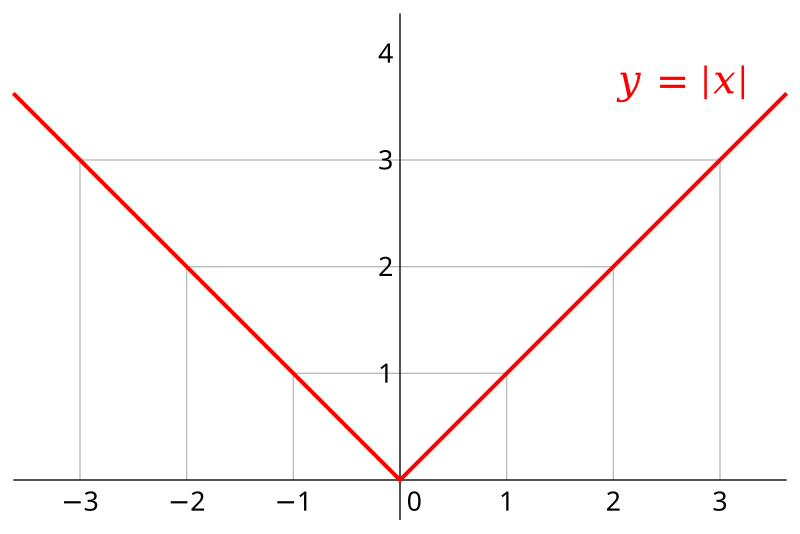
\includegraphics[width=0.5\linewidth, height=5cm, keepaspectratio]{images/basic_math/Absolute_value.svg.png}
            \caption{Absolute Value function/ Modulus Function \cite{wiki/Absolute-value}}
        \end{figure}
    \end{minipage}
\end{table}

\begin{lstlisting}[
    language=Python, 
    caption=Absolute value function
]
def get_absolute_value(val):
    if val >= 0:
        return val
    else:
        return -1 * val
\end{lstlisting}

\subsection*{Properties}

\subsubsection*{Fundamental properties \cite{wiki/Absolute-value}} \label{Basic Functions/Absolute Value function or Modulus Function/Fundamental properties}

\begin{customArrayStretch}{1.2}
\begin{tabular}{r l l}
     1. & ${\displaystyle |a|\geq 0}$ & Non-negativity \\
     
     2. & ${\displaystyle |a|=0\iff a=0}$ & Positive-definiteness \\
     
     3. & ${\displaystyle |ab|=\left|a\right|\left|b\right|}$ & 	Multiplicativity \\
     
     4. & ${\displaystyle |a+b|\leq |a|+|b|}$ & 	Subadditivity, specifically the triangle inequality \\
\end{tabular}
\end{customArrayStretch}

\subsubsection*{Additional useful properties \cite{wiki/Absolute-value}} \label{Basic Functions/Absolute Value function or Modulus Function/Additional useful properties}

\begin{customArrayStretch}{1.5}
\begin{tabular}{r l p{13cm}}
     1. & ${\displaystyle {\bigl |}\left|a\right|{\bigr |}=|a|}$ & 	Idempotence (the absolute value of the absolute value is the absolute value) \\
     
     2. & ${\displaystyle \left|-a\right|=|a|}$ & Evenness (reflection symmetry of the graph) \\
     
     3. & ${\displaystyle |a-b|=0\iff a=b}$ & 	Identity of indiscernibles (equivalent to positive-definiteness) \\
     
     4. & ${\displaystyle |a-b|\leq |a-c|+|c-b|}$ & 	Triangle inequality (equivalent to subadditivity) \\
     
     5. & ${\displaystyle \left|{\frac {a}{b}}\right|={\frac {|a|}{|b|}}\ }$ (if ${\displaystyle b\neq 0}$) & 	Preservation of division (equivalent to multiplicativity) \\
     
     6. & ${\displaystyle |a-b|\geq {\bigl |}\left|a\right|-\left|b\right|{\bigr |}}$ & 	Reverse triangle inequality (equivalent to subadditivity) \\
\end{tabular}
\end{customArrayStretch}

\subsection*{Inequalities} \label{Basic Functions/Absolute Value function or Modulus Function/Inequalities}

\begin{enumerate}
    \item ${\displaystyle |a|\leq b\iff -b\leq a\leq b}$

    \item ${\displaystyle |a|\geq b\iff b\leq a\leq -b\ }$

\end{enumerate}

\subsection*{Derivative} \label{Basic Functions/Absolute Value function or Modulus Function/Derivative}

\begin{enumerate}
    \item $
        {\displaystyle {\frac {d\left|x\right|}{dx}}={\frac {x}{|x|}}={\begin{cases}-1&x<0\\1&x>0\end{cases}}}
    $

    \item $
        {\displaystyle {d \over dx}f(|x|)={x \over |x|}(f'(|x|))}
    $ \hfill (discontinuous at $x=0$)

    \item $
        {\displaystyle {d \over dx}|f(x)|={f(x) \over |f(x)|}f'(x)}
    $ \hfill (discontinuous at $f(x)=0$)
\end{enumerate}


\subsection*{Anti-derivative/ Integral} \label{Basic Functions/Absolute Value function or Modulus Function/Anti-derivative or Integral}

$
    {\displaystyle \dint \left|x\right|dx={\dfrac {x\left|x\right|}{2}}+C}
$






\partition{Data}
\chapter{Data}

\section{Measurement Levels \cite{statistics/book/Statistics-for-Data-Scientists/Maurits-Kaptein}}\label{Data/Measurement-Levels}

\subsection{Nominal, Ordinal, Interval and Ratio \cite{statistics/book/Statistics-for-Data-Scientists/Maurits-Kaptein}}\label{Data/Measurement-Levels/Nominal, Ordinal, Interval and Ratio}

\label{Data/Measurement-Levels/Nominal, Ordinal, Interval and Ratio/Categorical Data}
\label{Data/Measurement-Levels/Nominal, Ordinal, Interval and Ratio/Numerical Data}
\label{Data/Measurement-Levels/Nominal, Ordinal, Interval and Ratio/Nominal}
\label{Data/Measurement-Levels/Nominal, Ordinal, Interval and Ratio/Ordinal}
\label{Data/Measurement-Levels/Nominal, Ordinal, Interval and Ratio/Interval}
\label{Data/Measurement-Levels/Nominal, Ordinal, Interval and Ratio/Ratio}

\begin{table}[H]
    \hfill
    \begin{minipage}[H]{0.25\linewidth}
        \textbf{Levels}: \cite{statistics/book/Statistics-for-Data-Scientists/Maurits-Kaptein}
        \begin{enumerate}
            \item Nominal
            \item Ordinal
            \item Interval
            \item Ratio
        \end{enumerate}
    \end{minipage}
    \hfill
    \begin{minipage}[H]{0.65\linewidth}
        \begin{table}[H]
            \centering
            \begin{tabular}{|p{5cm}|c|c|c|c|}
                \hline
                & \multicolumn{2}{c|}{\textbf{Categorical Data}} & \multicolumn{2}{c|}{\textbf{Numerical Data}} \\ 
                
                \hline
                & \textbf{Nominal} & \textbf{Ordinal} & \textbf{Interval} & \textbf{Ratio} \\ \hline
                
                Distinction between groups / individuals & \checkmark & \checkmark & \checkmark & \checkmark \\ \hline
                
                Imposes logical Order & \xmark & \checkmark & \checkmark & \checkmark \\ \hline
                
                Provides a magnitude of the differences in some unit & \xmark & \xmark & \checkmark & \checkmark \\ \hline
                
                A clear reference point or "0" & \xmark & \xmark & \xmark & \checkmark \\ \hline
            \end{tabular}
            \caption{Data: Measurement Levels: Nominal, Ordinal, Interval and Ratio \cite{statistics/book/Statistics-for-Data-Scientists/Maurits-Kaptein}}
        \end{table}
    \end{minipage}
    \hfill
\end{table}

\vspace{0.3cm}

\textbf{Note}:
\begin{enumerate}
    \item Each consecutive measurement level contains as much "information" - in a fairly loose sense of the word - as the previous one and more. \cite{statistics/book/Statistics-for-Data-Scientists/Maurits-Kaptein}
\end{enumerate}


\subsection{Continuous vs Discrete numerical data \cite{statistics/book/Statistics-for-Data-Scientists/Maurits-Kaptein}}\label{Data/Measurement-Levels/Continuous vs Discrete numerical data}

\label{Data/Measurement-Levels/Continuous vs Discrete numerical data/Continuous numerical data}
\label{Data/Measurement-Levels/Continuous vs Discrete numerical data/Discrete numerical data}

\begin{enumerate}
    \item Continuous variables can assume any value.\\
    This means that the continuous variable can attain any value between two different values, no matter how close the two values are.\\
    \textbf{Example}: temperature, weight, and age

    \item Discrete variables cannot assume any value between 2 values\\
    \textbf{Example}: number of text messages, accidents, microorganisms, students, etc.
\end{enumerate}


\subsection{Outliers \cite{statistics/book/Statistics-for-Data-Scientists/Maurits-Kaptein}}\label{Data/Measurement-Levels/Outliers}

\begin{enumerate}
    \item An outlier is a data point that significantly deviates from other observations in a dataset. \cite{common/online/chatgpt}

    \item Caused by Natural variability in the data or measurement errors. \cite{common/online/chatgpt}

    \item Typically identified using statistical methods like the IQR (Interquartile Range), Z-score, or visualization techniques (e.g., box plots). \cite{common/online/chatgpt}

    \item Outliers are not necessarily incorrect; they may represent rare but valid observations. \cite{common/online/chatgpt}
    
\end{enumerate}


\vspace{0.3cm}

\textbf{Examples}:
\begin{enumerate}
    \item In a dataset of human heights, a person measuring 250 cm might be an outlier but not necessarily unrealistic if it’s a rare case of gigantism. \cite{common/online/chatgpt}
\end{enumerate}


\vspace{0.3cm}
\textbf{Handling/ Dealing with Outliers}:
\begin{enumerate}
    \item Ignore these abnormalities and go ahead with the data. \cite{statistics/book/Statistics-for-Data-Scientists/Maurits-Kaptein}

    \item Delete/ remove the suspected records/ entries. \cite{statistics/book/Statistics-for-Data-Scientists/Maurits-Kaptein}

    \item Substitute them, using statistical methods, with a more plausible alternative. (aka \textbf{imputation}) \cite{statistics/book/Statistics-for-Data-Scientists/Maurits-Kaptein}\label{Data/Outliers/imputation}
\end{enumerate}




\subsection{Unrealistic Values \cite{statistics/book/Statistics-for-Data-Scientists/Maurits-Kaptein}}\label{Data/Measurement-Levels/Unrealistic Values}

\begin{enumerate}
    \item An unrealistic value is a data point that is not plausible within the context of the dataset, often due to data entry errors or faulty sensors. \cite{common/online/chatgpt}

    \item Caused by Human error, sensor malfunction, or corruption during data transmission. \cite{common/online/chatgpt}

    \item Typically identified using domain knowledge or logical constraints. \cite{common/online/chatgpt}

    \item Unlike outliers, unrealistic values are generally not useful and need correction or removal. \cite{common/online/chatgpt}

\end{enumerate}

\vspace{0.3cm}

\textbf{Examples}:
\begin{enumerate}
    \item A recorded body temperature of 200°C for a human is unrealistic, as it’s physically impossible for a person to survive at that temperature. \cite{common/online/chatgpt}

    \item Negative age of a person \cite{common/online/chatgpt}

    \item Missing values \cite{statistics/book/Statistics-for-Data-Scientists/Maurits-Kaptein}

    \item Incorrect datatype of value \cite{statistics/book/Statistics-for-Data-Scientists/Maurits-Kaptein}
\end{enumerate}

\vspace{0.3cm}
\textbf{Handling/ Dealing with Unrealistic values}:
\begin{enumerate}
    \item Delete/ remove the suspected records/ entries. \cite{statistics/book/Statistics-for-Data-Scientists/Maurits-Kaptein}
    
\end{enumerate}





\section{Describing Data \cite{statistics/book/Statistics-for-Data-Scientists/Maurits-Kaptein}} \label{Data/Describing Data}

Some \textbf{descriptive statistics}\label{Data/Describing Data/descriptive statistics} (or just \textbf{descriptives}\label{Data/Describing Data/descriptives}) that we introduce are often used for data of a certain measurement level. \cite{statistics/book/Statistics-for-Data-Scientists/Maurits-Kaptein}

\subsection{Frequency/ Frequency table \cite{statistics/book/Statistics-for-Data-Scientists/Maurits-Kaptein}}\label{Data/Describing Data/Frequency or Frequency table}

\textbf{Measurement levels}: Nominal and ordinal data

\vspace{0.3cm}

\begin{enumerate}
    \item Frequencies are often uninformative for interval or ratio variables. \cite{statistics/book/Statistics-for-Data-Scientists/Maurits-Kaptein}\\
        if there are lots and lots of different possible values, all of them will have a count of just one. \cite{statistics/book/Statistics-for-Data-Scientists/Maurits-Kaptein}\\
        This is often tackled by discretizing (or "\textbf{binning}”\label{Data/Describing Data/Frequency or Frequency table/binning}) the variable (which, note, effectively "throws away” some of the information in the data). \cite{statistics/book/Statistics-for-Data-Scientists/Maurits-Kaptein}

    
\end{enumerate}


\subsubsection{(Absolute) Frequency/ (Absolute) Frequency table \cite{statistics/book/Statistics-for-Data-Scientists/Maurits-Kaptein}}\label{Data/Describing Data/Frequency or Frequency table/Absolute}

\begin{enumerate}
    \item It refers to the count of occurrences of a particular value or category in a dataset. \cite{common/online/chatgpt}

    \item Simple count, no further processing. \cite{common/online/chatgpt}

    \item \textbf{Use Case}: Helpful in creating bar charts or histograms. \cite{common/online/chatgpt}
\end{enumerate}



\subsubsection{Cumulative Frequency/ Cumulative Frequency table \cite{statistics/book/Statistics-for-Data-Scientists/Maurits-Kaptein}}\label{Data/Describing Data/Frequency or Frequency table/Cumulative}

\begin{enumerate}
    \item It is the running total of frequencies up to a certain value or class. \cite{common/online/chatgpt}

    \item Each cumulative frequency includes its own frequency plus all previous frequencies. \cite{common/online/chatgpt}

    \item \textbf{Use Case}: Useful in percentile calculations and ogive graphs. \cite{common/online/chatgpt}

    \item The cumulative frequency makes more sense for ordinal data than for nominal data, since ordinal data can be ordered in size, which is not possible for nominal data. \cite{statistics/book/Statistics-for-Data-Scientists/Maurits-Kaptein}
\end{enumerate}

\begin{table}[H]
    \begin{minipage}[H]{0.3\linewidth}
    $
        \begin{aligned}
            CF_i 
                &= CF_{i-1} + F_{i} \\
                &= \sum_{k=1}^{i} F_{k}
        \end{aligned}
    $
    \end{minipage}
    \begin{minipage}[H]{0.65\linewidth}
        \begin{table}[H]
            \begin{tabular}{l l}
                $CF_i$ & Cumulative Frequency at the current value \\ 
                $CF_{i-1}$ & Cumulative Frequency at the previous value \\ 
                $F_i$ & Frequency at the current value \\ 
            \end{tabular}
            \caption*{Notations}
        \end{table}
    \end{minipage}
\end{table}


\subsubsection{Relative Frequency/ Relative Frequency table \cite{statistics/book/Statistics-for-Data-Scientists/Maurits-Kaptein}}\label{Data/Describing Data/Frequency or Frequency table/Relative}

\begin{enumerate}
    \item It shows the proportion of each category relative to the total number of observations. \cite{common/online/chatgpt}

    \item Expressed as a fraction, decimal, or percentage. \cite{common/online/chatgpt}

    \item \textbf{Use Case}: Ideal for creating pie charts and understanding distribution proportions. \cite{common/online/chatgpt}
\end{enumerate}


\begin{table}[H]
    \begin{minipage}{0.3\linewidth}
        \[
            \begin{aligned}
                RF_i 
                    &= \dfrac{F_{i}}{\dsum_{k=1}^{N} F_{k}}
            \end{aligned}
        \]
    \end{minipage}
    \begin{minipage}{0.65\linewidth}
        \begin{table}[H]
            \begin{tabular}{l l}
                $RF_i$ & Relative Frequency \\
                $F_i$ & Frequency of the value \\ 
                $N$ & Total number of observations \\ 
            \end{tabular}
            \caption*{Notations}
        \end{table}
    \end{minipage}
\end{table}




\subsubsection{Cumulative Relative Frequency/ Cumulative Relative Frequency table \cite{statistics/book/Statistics-for-Data-Scientists/Maurits-Kaptein}}\label{Data/Describing Data/Frequency or Frequency table/Cumulative Relative}

\begin{enumerate}
    \item Cumulative relative frequency is the accumulation of the relative frequencies of data points up to a certain value. \cite{common/online/chatgpt}

    \item It indicates the proportion of data points that are less than or equal to a particular value. \cite{common/online/chatgpt}

    \item \textbf{Use Cases}:
    \begin{enumerate}
        \item Identifying percentiles and median.

        \item Visualizing with a cumulative relative frequency graph (Ogive).

        \item Understanding data distribution by determining the proportion of values below a specific threshold.
    \end{enumerate}
\end{enumerate}



\begin{table}[H]
    \begin{minipage}{0.3\linewidth}
        \[
            \begin{aligned}
                CRF_i 
                    &= \dfrac{\dsum_{k=1}^{i} F_{k}}{\dsum_{k=1}^{N} F_{k}}
            \end{aligned}
        \]
    \end{minipage}
    \begin{minipage}{0.65\linewidth}
        \begin{table}[H]
            \begin{tabular}{l l}
                $CRF_i$ & Cumulative Relative Frequency \\
                $F_i$ & Frequency of the value \\ 
                $N$ & Total number of observations \\ 
            \end{tabular}
            \caption*{Notations}
        \end{table}
    \end{minipage}
\end{table}





\subsection{Central Tendency \cite{statistics/book/Statistics-for-Data-Scientists/Maurits-Kaptein}}\label{Data/Describing Data/Central Tendency}

\begin{enumerate}
     \item When we work with numerical data, we often want to know something about the "central value" or "middle value" of the variable, also referred to as the \textbf{location}\label{Data/Describing Data/Central Tendency/location} of the data. \cite{statistics/book/Statistics-for-Data-Scientists/Maurits-Kaptein}
\end{enumerate}


\subsubsection{(Arithmetic) mean/ average \cite{statistics/book/Statistics-for-Data-Scientists/Maurits-Kaptein}} \label{Data/Describing Data/Central Tendency/(Arithmetic) mean or average}

\begin{table}[H]
    \begin{minipage}{0.3\linewidth}
        $
            \bar{x} = \dfrac{1}{n} \dsum_{i=1}^{n} x_i
        $
    \end{minipage}
    \begin{minipage}{0.65\linewidth}
        \begin{table}[H]
            \begin{tabular}{l l}
                $\bar{x}$ & mean \\
                $x_i$ & item \\
                $n$ & number of items \\
            \end{tabular}
            \caption*{Notations}
        \end{table}
    \end{minipage}
\end{table}



\subsubsection{Mode \cite{statistics/book/Statistics-for-Data-Scientists/Maurits-Kaptein}} \label{Data/Describing Data/Central Tendency/Mode}

\begin{enumerate}
    \item The mode is merely the most frequently occurring value. \cite{statistics/book/Statistics-for-Data-Scientists/Maurits-Kaptein}

    \item There might be multiple modes. \cite{statistics/book/Statistics-for-Data-Scientists/Maurits-Kaptein}
    
\end{enumerate}



\subsubsection{Median \cite{statistics/book/Statistics-for-Data-Scientists/Maurits-Kaptein}} \label{Data/Describing Data/Central Tendency/Median}

\begin{enumerate}
    \item The median is a value that divides the ordered data from small to large (or large to small) into two equal parts: 50\% of the data is below the median and 50\% is above. \cite{statistics/book/Statistics-for-Data-Scientists/Maurits-Kaptein}

    \item The median is not necessarily a value that is present in the data. \cite{statistics/book/Statistics-for-Data-Scientists/Maurits-Kaptein}
\end{enumerate}


\vspace{0.3cm}
\textbf{Steps}:
\begin{enumerate}
    \item sort the data

    \item choose the middle-most value when $n$ is \textbf{odd}\\
        average of the two middle values when $n$ is \textbf{even}
\end{enumerate}



\subsubsection{Quantiles \cite{statistics/book/Statistics-for-Data-Scientists/Maurits-Kaptein}} \label{Data/Describing Data/Central Tendency/Quantiles}

\begin{enumerate}
    \item A quantile $x_q$ is a value that splits the ordered data of a variable $x$ into two parts: \cite{statistics/book/Statistics-for-Data-Scientists/Maurits-Kaptein}
    \begin{enumerate}
        \item $q \cdot 100\%$ of the data is below the value $x_q$

        \item $(1 - q) \cdot 100\%$ of the data is above the value $x_q$
    \end{enumerate}
    
    \item The parameter $q$ can take any value in the interval $[0, 1]$. \cite{statistics/book/Statistics-for-Data-Scientists/Maurits-Kaptein}

    \item Quantiles can be calculated in different ways, depending on the way we "interpolate" between two values. \cite{statistics/book/Statistics-for-Data-Scientists/Maurits-Kaptein} \\
    We could map the ordered values \textit{equally spaced} on the interval $(0, 1)$, where the \textit{i}th ordered value of the data is positioned at the level $q_i = {i}/{(n + 1)}$ in the interval $(0, 1)$, with $n$ being the number of data points. \cite{statistics/book/Statistics-for-Data-Scientists/Maurits-Kaptein} \\
    R uses $q_i = (i - 1)/(n - 1)$ for quantiles. \cite{statistics/book/Statistics-for-Data-Scientists/Maurits-Kaptein} \\
    \textbf{Example}: \cite{statistics/book/Statistics-for-Data-Scientists/Maurits-Kaptein}
    \begin{enumerate}
        \item Data points: $\dCurlyBrac{2, 5, 6, 4}$ ($n=4$)
        \item Sorted Data points: $\dCurlyBrac{2, 4, 5, 6}$ ($n=4$)
        \item Quantiles:\\[0.2cm]
        \begin{tabular}{|l|c|c|c|}
            \hline
            $i$ & $x_i$ & $q_i = i/(n+1) = i/5$ & $q_i = (i-1)/(n-1) = (i-1)/3$ \\ [0.1cm]
            \hline
            $1$ & $2$ & $1/5 = 0.2$ & $0$ \\
            $2$ & $4$ & $2/5 = 0.4$ & $1/3$ \\
            $3$ & $5$ & $3/5 = 0.6$ & $2/3$ \\
            $4$ & $6$ & $4/5 = 0.8$ & $1$ \\
            \hline
        \end{tabular}\\

        \item If $x_i = 3 \Rightarrow q_i = 0.3$
    \end{enumerate}
\end{enumerate}




\subsubsection{Quartiles \cite{statistics/book/Statistics-for-Data-Scientists/Maurits-Kaptein}} \label{Data/Describing Data/Central Tendency/Quartiles}

\begin{enumerate}
    \item When $q = 0.25$, $q = 0.50$, and $q = 0.75$ the quantiles are referred to as the first, second, and third quartiles, respectively. \cite{statistics/book/Statistics-for-Data-Scientists/Maurits-Kaptein}
    \label{Data/Describing Data/Central Tendency/Quartiles/first quartile}
    \label{Data/Describing Data/Central Tendency/Quartiles/second quartile}
    \label{Data/Describing Data/Central Tendency/Quartiles/third quartile}

    \item Splits: \\
    \begin{tabular}{r l l l} % Right-align first column, left-align second column
        1. & $q = 0$ & to & $q = 0.25$ \\
        2. & $q = 0.25$ & to & $q = 0.5$ \\
        3. & $q = 0.5$ & to & $q = 0.75$ \\
        4. & $q = 0.75$ & to & $q = 1$ \\
    \end{tabular}
\end{enumerate}



\subsubsection{Deciles \cite{statistics/book/Statistics-for-Data-Scientists/Maurits-Kaptein}} \label{Data/Describing Data/Central Tendency/Deciles}

\begin{enumerate}
    \item We call quantiles deciles when $q$ is restricted to the set $\dCurlyBrac{0.1, 0.2,\cdots, 0.9}$

    \item Splits: \\
    \begin{tabular}{r l l l} % Right-align first column, left-align second column
        1. & $q = 0$ & to & $q = 0.1$ \\
        2. & $q = 0.1$ & to & $q = 0.2$ \\
        && \vdots & \\
        9. & $q = 0.8$ & to & $q = 0.9$ \\
        10. & $q = 0.9$ & to & $q = 1$ \\
    \end{tabular}
\end{enumerate}



\subsubsection{Percentiles \cite{statistics/book/Statistics-for-Data-Scientists/Maurits-Kaptein}} \label{Data/Describing Data/Central Tendency/Percentiles}

\begin{enumerate}
    \item We call quantiles percentiles when $q$ is restricted to the set $\dCurlyBrac{0.01, 0.02,\cdots, 0.99}$

    \item Splits: \\
    \begin{tabular}{r l l l} % Right-align first column, left-align second column
        1. & $q = 0$ & to & $q = 0.01$ \\
        2. & $q = 0.01$ & to & $q = 0.02$ \\
        & & \vdots & \\
        99. & $q = 0.98$ & to & $q = 0.99$ \\
        100. & $q = 0.99$ & to & $q = 1$ \\
    \end{tabular}
\end{enumerate}









\chapter{Visualizing Data} \label{Visualizing Data}

\begin{enumerate}
    \item Visualization, when done well, can make large and even high-dimensional datasets (relatively) easy to interpret. \hfill \cite{statistics/book/Statistics-for-Data-Scientists/Maurits-Kaptein}

    
\end{enumerate}


\begin{lstlisting}[
    language=Python
]
import random
import faker                    # to generate fake data
import numpy as np
import pandas as pd
from tqdm import tqdm           # progress bar

# plotting libraries
import seaborn as sns           
import matplotlib.pyplot as plt

random.seed(0)
np.random.seed(0)
faker.Faker.seed(0)

fake = faker.Faker()
\end{lstlisting}


\clearpage
\section{Box and Whiskers Plot/ Box Plot \cite{data/online/seaborn.boxplot, data/online/matplotlib.pyplot.boxplot}} \label{Visualizing Data/Box and Whiskers Plot or Box Plot}

\begin{lstlisting}[numbers=none]

                     Q1-1.5IQR   Q1   median  Q3   Q3+1.5IQR
                                  |-----:-----|
                  o      |--------|     :     |--------|    o  o
                                  |-----:-----|
                flier             <----------->            fliers
                                       IQR

\end{lstlisting}

\vspace{0.5cm}

\begin{table}[H]
\begin{minipage}[t]{0.35\linewidth}
\begin{figure}[H]
    \centering
    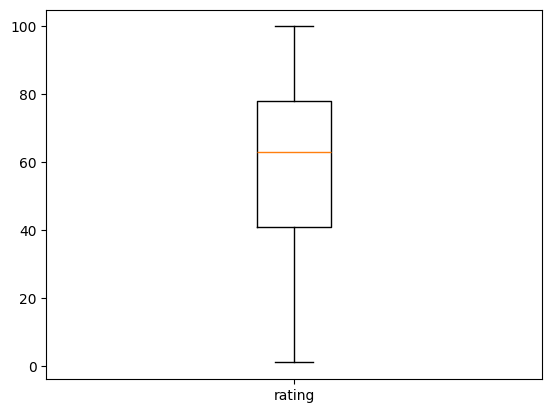
\includegraphics[width=0.9\linewidth, height=10cm, keepaspectratio]{images/data/__visualizations__/plt-box-rating-face-data.png}
    \caption{Box and Whiskers plot (py-plt) output (face\_data.csv)}
\end{figure}
\end{minipage}
\hspace{0.2cm}
\vrule width 1pt
\hspace{0.5cm}
\begin{minipage}[t]{0.57\linewidth}
\begin{lstlisting}[
    language=Python,
    caption=Box and Whiskers Plot: py-plt: face\_data.csv
]
_col = "rating"

plt.boxplot(df[_col])
plt.xticks([1], [_col])
plt.show()
\end{lstlisting}
\end{minipage}
\end{table}



\begin{table}[H]
\begin{minipage}[t]{0.35\linewidth}
\begin{figure}[H]
    \centering
    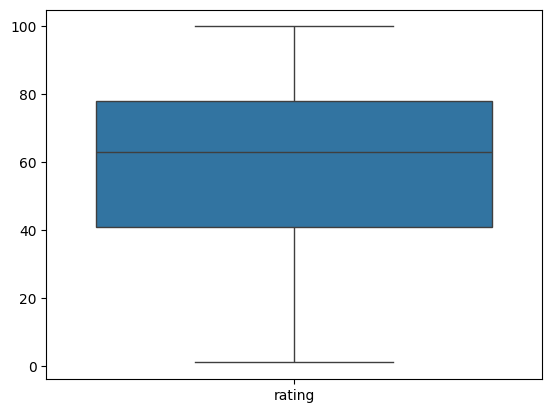
\includegraphics[width=0.9\linewidth, height=10cm, keepaspectratio]{images/data/__visualizations__/sns-box-rating-face-data.png}
    \caption{Box and Whiskers plot (py-sns) output (face\_data.csv)}
\end{figure}
\end{minipage}
\hspace{0.2cm}
\vrule width 1pt
\hspace{0.5cm}
\begin{minipage}[t]{0.57\linewidth}
\begin{lstlisting}[
    language=Python,
    caption=Box and Whiskers Plot: py-sns: face\_data.csv
]
_col = "rating"

sns.boxplot(df[_col])
plt.ylabel("")
plt.xticks([0], [_col])
plt.show()
\end{lstlisting}
\end{minipage}
\end{table}




\begin{enumerate}
    \item A box plot (or box-and-whisker plot) shows the distribution of quantitative data in a way that facilitates comparisons between variables or across levels of a categorical variable.  \hfill \cite{data/online/seaborn.boxplot}
    
    \item The box shows the quartiles of the dataset while the whiskers extend to show the rest of the distribution, except for points that are determined to be “outliers” using a method that is a function of the inter-quartile range. \hfill \cite{data/online/seaborn.boxplot}
\end{enumerate}





\clearpage
\section{Count Plot \cite{data/online/seaborn.countplot}} \label{Visualizing Data/Count Plot}


\begin{table}[H]
\begin{minipage}[t]{0.35\linewidth}
\begin{figure}[H]
    \centering
    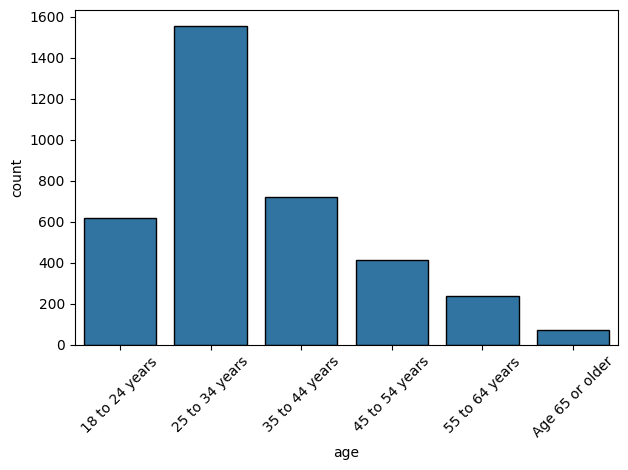
\includegraphics[width=0.9\linewidth, height=10cm, keepaspectratio]{images/data/__visualizations__/sns-countplot-face-data.png}
    \caption{Count plot (py-sns) output (face\_data.csv)}
\end{figure}
\end{minipage}
\hspace{0.2cm}
\vrule width 1pt
\hspace{0.5cm}
\begin{minipage}[t]{0.57\linewidth}
\begin{lstlisting}[
    language=Python,
    caption=Count Plot: py-sns: face\_data.csv
]
vals = df[df["age"] != " "].copy()

sns.countplot(
    x='age', 
    data=vals, 
    order=sorted(vals['age'].unique()), 
    edgecolor='black',
)

plt.xticks(rotation=45)
plt.tight_layout()
plt.show()
\end{lstlisting}
\end{minipage}
\end{table}

\vspace{0.3cm}

\begin{enumerate}
    \item Show the counts of observations in each categorical bin using bars.

    
\end{enumerate}



% \clearpage
\section{Density Plot \cite{data/online/seaborn.displot}} \label{Visualizing Data/Density Plot}

\begin{table}[H]
\begin{minipage}[t]{0.35\linewidth}
\begin{figure}[H]
    \centering
    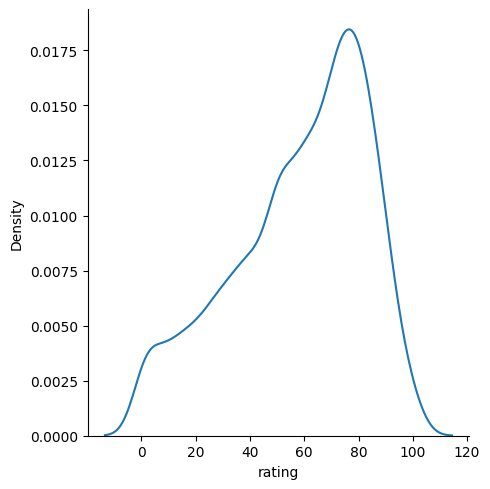
\includegraphics[width=0.9\linewidth, height=10cm, keepaspectratio]{images/data/__visualizations__/sns-density-kde-rating-face-data.png}
    \caption{Density plot (py-sns) output (face\_data.csv)}
\end{figure}
\end{minipage}
\hspace{0.2cm}
\vrule width 1pt
\hspace{0.5cm}
\begin{minipage}[t]{0.57\linewidth}
\begin{lstlisting}[
    language=Python,
    caption=Density Plot: py-sns: face\_data.csv
]
sns.displot(df["rating"], kind="kde")

plt.show()
\end{lstlisting}

\vspace{0.2cm}

\begin{enumerate}
    \item A density plot - at least in this setting - can be considered a “continuous approximation” of a histogram. \hfill \cite{statistics/book/Statistics-for-Data-Scientists/Maurits-Kaptein} \\
    SEE: \fullref{Visualizing Data/Histogram}

    \item It gives per range of values of the continuous variable the probability of observing a value within that range. \hfill \cite{statistics/book/Statistics-for-Data-Scientists/Maurits-Kaptein}


\end{enumerate}

\end{minipage}
\end{table}







\clearpage
\section{Histogram \cite{data/online/seaborn.histplot}} \label{Visualizing Data/Histogram}


\begin{table}[H]
\begin{minipage}[t]{0.35\linewidth}
\begin{figure}[H]
    \centering
    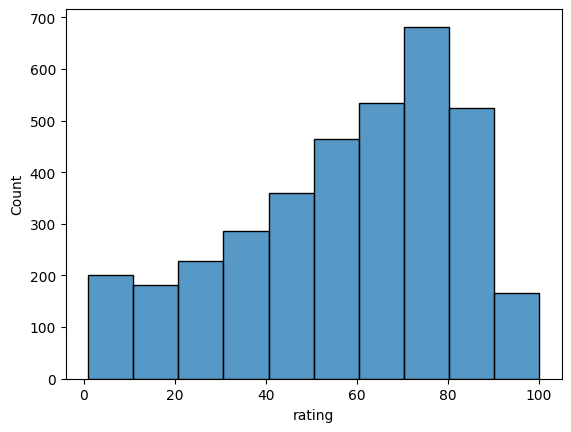
\includegraphics[width=0.9\linewidth, height=10cm, keepaspectratio]{images/data/__visualizations__/sns-hist-rating-face-data.png}
    \caption{Histogram (py-sns) output (face\_data.csv)}
\end{figure}
\end{minipage}
\hspace{0.2cm}
\vrule width 1pt
\hspace{0.5cm}
\begin{minipage}[t]{0.57\linewidth}
\begin{lstlisting}[
    language=Python,
    caption=Histogram: py-sns: face\_data.csv
]
sns.histplot(df["rating"], binwidth=10)
plt.show()
\end{lstlisting}

\vspace{0.2cm}

\begin{enumerate}
    \item A histogram is a classic visualization tool that represents the distribution of one or more variables by counting the number of observations that fall within discrete bins. \hfill \cite{data/online/seaborn.histplot}

    \item A histogram “bins” the data (discretizes it), and subsequently shows the frequency of occurrence in each bin. \hfill \cite{statistics/book/Statistics-for-Data-Scientists/Maurits-Kaptein}
    
    \item It is the continuous variant of the bar chart. \hfill \cite{statistics/book/Statistics-for-Data-Scientists/Maurits-Kaptein}\\
    SEE: \fullref{Visualizing Data/Box and Whiskers Plot or Box Plot}
    
    \item The number of bins selected makes a big difference in the visualization: too few bins obscure the patterns in the data, but too many bins lead to counts of exactly one for each value. \hfill \cite{statistics/book/Statistics-for-Data-Scientists/Maurits-Kaptein}
\end{enumerate}

\end{minipage}
\end{table}


% \clearpage
\section{Pairwise Plot \cite{statistics/book/Statistics-for-Data-Scientists/Maurits-Kaptein, data/online/seaborn.pairplot}} \label{Visualizing Data/Pairwise Plot}


\begin{table}[H]
\begin{minipage}[t]{0.35\linewidth}
\begin{figure}[H]
    \centering
    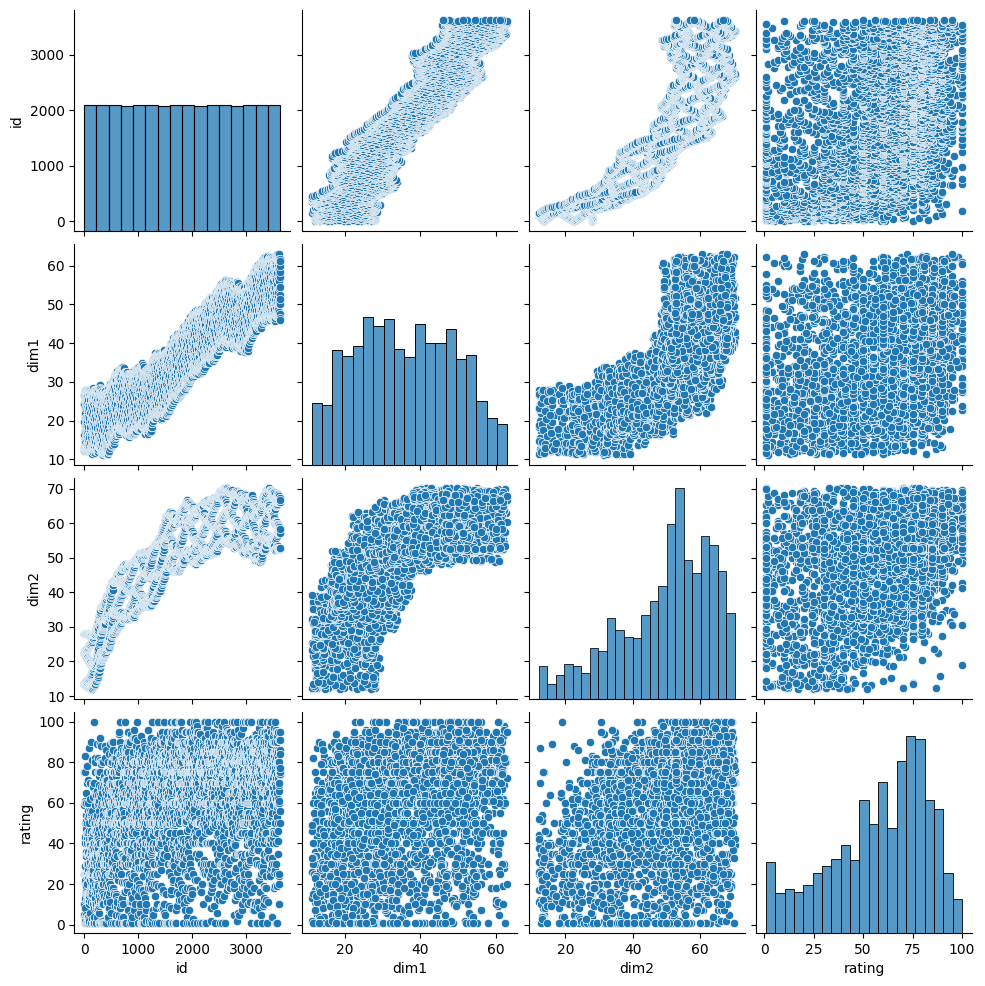
\includegraphics[width=0.9\linewidth, height=10cm, keepaspectratio]{images/data/__visualizations__/sns-pairplot-face-data.png}
    \caption{Pairwise plot (py-sns) output (face\_data.csv)}
\end{figure}
\end{minipage}
\hspace{0.2cm}
\vrule width 1pt
\hspace{0.5cm}
\begin{minipage}[t]{0.57\linewidth}
\begin{lstlisting}[
    language=Python,
    caption=Pairwise Plot: py-sns: face\_data.csv
]
df = pd.read_csv("face_data.csv")
sns.pairplot(df)
\end{lstlisting}

\vspace{0.3cm}

\begin{enumerate}
    \item Plot pairwise relationships in a dataset. \hfill \cite{data/online/seaborn.pairplot}

    \item By default, this is a grid of Axes such that each numeric variable in data will by shared across the y-axes across a single row and the x-axes across a single column. \hfill \cite{data/online/seaborn.pairplot}
    
    \item The diagonal plots are treated differently: a univariate distribution plot is drawn to show the marginal distribution of the data in each column. \hfill \cite{data/online/seaborn.pairplot}
\end{enumerate}
\end{minipage}
\end{table}











\clearpage
\section{Pie Chart \cite{data/online/matplotlib.pyplot.pie}} \label{Visualizing Data/Pie Chart}


\begin{table}[H]
\begin{minipage}[t]{0.35\linewidth}
\begin{figure}[H]
    \centering
    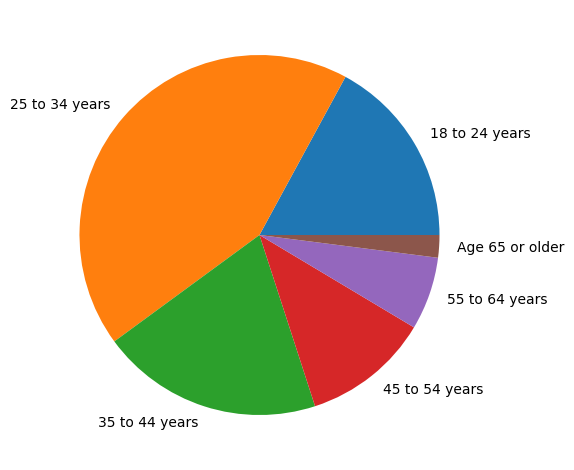
\includegraphics[width=0.9\linewidth, height=10cm, keepaspectratio]{images/data/__visualizations__/plt-pie-age-face-data.png}
    \caption{Pie chart (py-plt) output (face\_data.csv)}
\end{figure}
\end{minipage}
\hspace{0.2cm}
\vrule width 1pt
\hspace{0.5cm}
\begin{minipage}[t]{0.57\linewidth}
\begin{lstlisting}[
    language=Python,
    caption=Pie Chart: py-plt: face\_data.csv
]
vals = df[df["age"] != " "].copy()

labels, counts = np.unique(
    vals['age'],
    return_counts=True
)

plt.pie(counts, labels=labels)

plt.tight_layout()
plt.show()
\end{lstlisting}
\end{minipage}
\end{table}



\clearpage
\section{Scatter Plot \cite{data/online/seaborn.scatterplot, data/online/seaborn.scatterplot, data/online/wiki/Scatter_plot}} \label{Visualizing Data/Scatter Plot}


\begin{table}[H]
\begin{minipage}[t]{0.35\linewidth}
\begin{figure}[H]
    \centering
    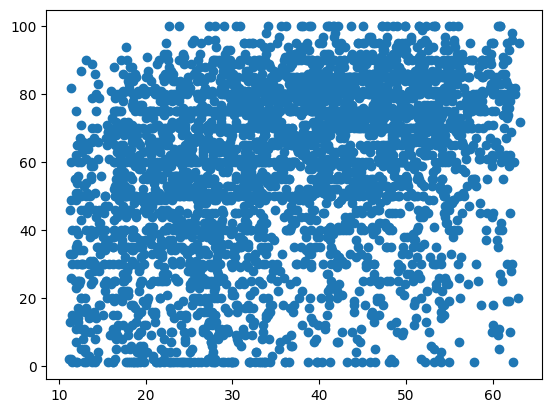
\includegraphics[width=0.9\linewidth, height=10cm, keepaspectratio]{images/data/__visualizations__/plt-scatter-dim1-rating-face-data.png}
    \caption{Scatter Plot (py-plt) output (face\_data.csv)}
\end{figure}
\end{minipage}
\hspace{0.2cm}
\vrule width 1pt
\hspace{0.5cm}
\begin{minipage}[t]{0.57\linewidth}
\begin{lstlisting}[
    language=Python,
    caption=Scatter Plot: py-plt: face\_data.csv
]
plt.scatter(df["dim1"], df["rating"])

plt.show()
\end{lstlisting}
\end{minipage}
\end{table}

\begin{table}[H]
\begin{minipage}[t]{0.35\linewidth}
\begin{figure}[H]
    \centering
    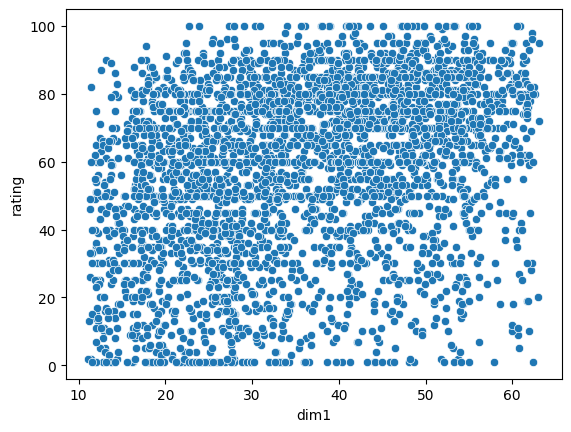
\includegraphics[width=0.9\linewidth, height=10cm, keepaspectratio]{images/data/__visualizations__/sns-scatter-dim1-rating-face-data.png}
    \caption{Scatter Plot (py-sns) output (face\_data.csv)}
\end{figure}
\end{minipage}
\hspace{0.2cm}
\vrule width 1pt
\hspace{0.5cm}
\begin{minipage}[t]{0.57\linewidth}
\begin{lstlisting}[
    language=Python,
    caption=Scatter Plot: py-sns: face\_data.csv
]
sns.scatterplot(df, x="dim1", y="rating")

plt.show()
\end{lstlisting}
\end{minipage}
\end{table}





\begin{enumerate}
    \item A scatter plot, also called a \textbf{scatterplot}, \textbf{scatter graph}\label{Visualizing Data/scatter graph}, \textbf{scatter chart}\label{Visualizing Data/scatter chart}, \textbf{scattergram}\label{Visualizing Data/scattergram}, or \textbf{scatter diagram}\label{Visualizing Data/scatter diagram}, is a type of plot or mathematical diagram using Cartesian coordinates to display values for typically two variables for a set of data. \hfill \cite{data/online/wiki/Scatter_plot}
    
    \item If the points are coded (color/shape/size), one additional variable can be displayed. \hfill \cite{data/online/wiki/Scatter_plot}
    
    \item The data are displayed as a collection of points, each having the value of one variable determining the position on the horizontal axis and the value of the other variable determining the position on the vertical axis. \hfill \cite{data/online/wiki/Scatter_plot}
\end{enumerate}











\partition{Mathematics: Statistics}
\chapter{Sampling Plans}\label{Sampling Plans}


\begin{figure}[H]
    \centering
    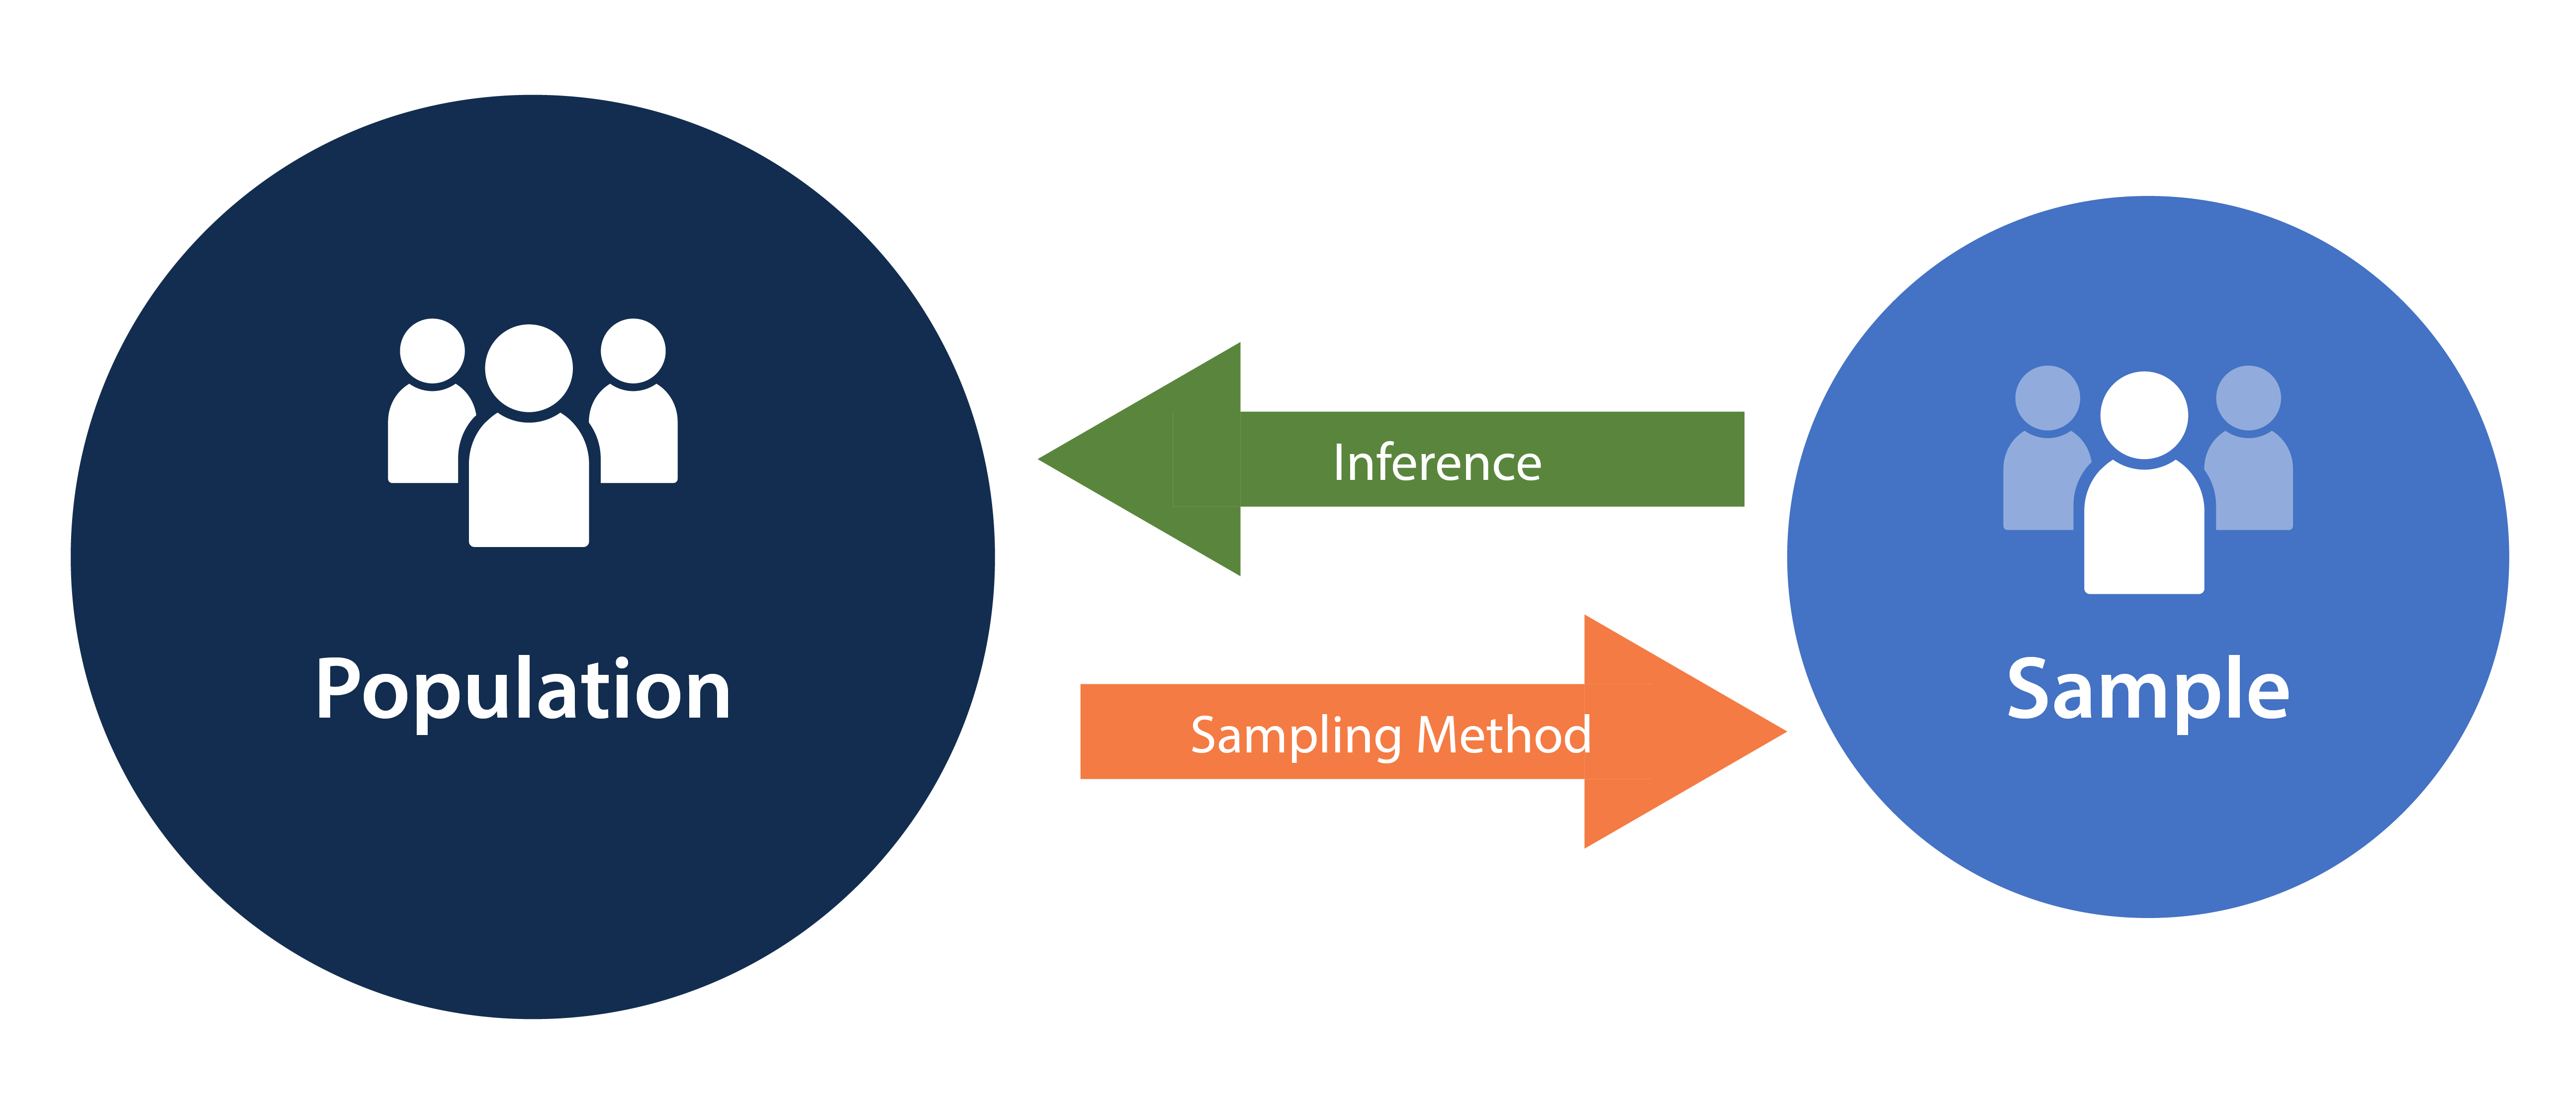
\includegraphics[
        width=0.5\linewidth,
        height=5cm,
        keepaspectratio
    ]{images/statistics/sampling-plan.png}

    \caption{Sampling Plan: Relation between Population and Sample}
\end{figure}


\begin{enumerate}
    \item \textbf{Statistical Inference}\label{Sampling Plans/Statistical Inference}: To extend your conclusions beyond the observed data.
    The field of \textbf{inferential statistics} tries to use the information from a sample to make statements or decisions about the population of interest.
    It takes into account the uncertainty that the information is coming from sampling and does not perfectly represent the population, since another sample would give different outcomes.
    An important aspect of inferential statistics is estimation of the population parameters of interest.
    \hfill \cite{statistics/book/Statistics-for-Data-Scientists/Maurits-Kaptein}

    \item Sampling procedures are formal \textit{probabilistic approaches} to help collect units from the population for the sample.
    \hfill \cite{statistics/book/Statistics-for-Data-Scientists/Maurits-Kaptein}

    \item \textbf{Population}\label{Sampling Plans/Population}: The complete set of units that we would like to say something about is called the (target) population.
    \hfill \cite{statistics/book/Statistics-for-Data-Scientists/Maurits-Kaptein}
    \\
    In principle we would expect that a population is \textbf{always finite}, since an infinite number of units does not exist in real life. However, populations are often treated as infinite. One reason is that populations can be really really large.
    \hfill \cite{statistics/book/Statistics-for-Data-Scientists/Maurits-Kaptein}
    \\
    It is mathematically often more convenient (as we will see later) to assume that such a population is infinite.
    \hfill \cite{statistics/book/Statistics-for-Data-Scientists/Maurits-Kaptein}
    \\
    Properly defining or describing a population can be difficult. Furthermore, even if the population is established, measuring all units is often impossible or too elaborate. This means that information about the population can only be obtained by considering a subset of the population.
    \hfill \cite{statistics/book/Statistics-for-Data-Scientists/Maurits-Kaptein}

    \item \textbf{Sample}\label{Sampling Plans/Sample}: The set of units for which we have obtained data is referred to as the sample.
    \hfill \cite{statistics/book/Statistics-for-Data-Scientists/Maurits-Kaptein}
    \\
    The sample is typically a subset of the population, although in theory the sample can form the whole population or the sample can contain units that are not from the target population.
    \hfill \cite{statistics/book/Statistics-for-Data-Scientists/Maurits-Kaptein}

    \item \textbf{Representative Sample}\label{Sampling Plans/Representative Sample}:  A representative sample can be intuitively defined as a sample of units that has approximately the same distribution of characteristics as the population from which it was drawn.
    \hfill \cite{statistics/book/Statistics-for-Data-Scientists/Maurits-Kaptein}
    \\
    Representative sampling is also referred to as random or probability sampling.
    \hfill \cite{statistics/book/Statistics-for-Data-Scientists/Maurits-Kaptein}

    \item \textbf{Unit}\label{Sampling Plans/Unit}: A unit is usually a concrete or physical thing for which we would like to measure its characteristics.
    \hfill \cite{statistics/book/Statistics-for-Data-Scientists/Maurits-Kaptein}

    \item \textbf{Estimates}\label{Sampling Plans/Estimates}: In terms of statistical inference, the calculations on the sample data are referred to as estimates for the theoretical value in the whole population.
    \hfill \cite{statistics/book/Statistics-for-Data-Scientists/Maurits-Kaptein}

    \item \textbf{Estimators}\label{Sampling Plans/Estimators}: quantities that we compute using the data in our sample to say something about the population.
    \hfill \cite{statistics/book/Statistics-for-Data-Scientists/Maurits-Kaptein}

    \item \textbf{Realization}\label{Sampling Plans/realization}: The values in the sample are referred to as a realization from the population.
    \hfill \cite{statistics/book/Statistics-for-Data-Scientists/Maurits-Kaptein}

    %%%%%%%%%%%%%%%%%%%%%%%%%%%%%%%%%%%%%%%%%%%%%%%%%%%%%%%%%%%%%%%%%%%%%%%%%%%%%%
    \vspace{0.5cm}

    \item Reasons for sample instead of population:
    \begin{enumerate}
        \item In many applications we really can’t measure the complete population. For instance, one of the tests applied to aircraft engines is the “frozen bird test”.
        \hfill \cite{statistics/book/Statistics-for-Data-Scientists/Maurits-Kaptein}

        \item Time, space, or budget restrictions often do not allow us to measure all units from a population.
        \hfill \cite{statistics/book/Statistics-for-Data-Scientists/Maurits-Kaptein}

        \item  Big data itself may be an argument for sampling. If we have a very large sample or we have been able to measure all units from the population, the resulting dataset can be so large that it becomes impossible to analyze the full data at one computer.
        \hfill \cite{statistics/book/Statistics-for-Data-Scientists/Maurits-Kaptein}
    \end{enumerate}

    \item A non-representative sample implies that we do not know the exact process by which units in the population became part of the sample.
    \hfill \cite{statistics/book/Statistics-for-Data-Scientists/Maurits-Kaptein}

    \item If we know which sampling procedure was applied to collect the units for the sample, we would also know how close the calculations or statistics would be to the theoretical value in the whole population.
    \hfill \cite{statistics/book/Statistics-for-Data-Scientists/Maurits-Kaptein}
    \\
    Thus the sampling procedure and the choice of calculation on the sample data (\\
    \nameref{Data/Describing Data/Central Tendency/(Arithmetic) mean or average}, \\
    \nameref{Data/Describing Data/Central Tendency/Median},\\
    \nameref{Data/Describing Data/Central Tendency/Quartiles/first quartile}, \\
    \nameref{Data/Describing Data/Central Tendency/Standard Deviation}\\
    etc.) would make statistical inference mathematically precise and it would therefore help us when making statements beyond the sample data.
    \hfill \cite{statistics/book/Statistics-for-Data-Scientists/Maurits-Kaptein}


\end{enumerate}

\section{Generic Formulation \cite{statistics/book/Statistics-for-Data-Scientists/Maurits-Kaptein}}

\begin{customArrayStretch}{1.3}
\begin{longtable}{>{\RaggedRight\arraybackslash}p{4cm} >{\centering\arraybackslash}p{0.5cm} p{10.5cm}}

\hhline{=:=:=} \endfirsthead
\hhline{=:=:=} \endhead
\hhline{=:=:=} \endfoot
\hhline{=:=:=} \endlastfoot


\textbf{Population Size} &
    $N$ &
    \hfill \cite{statistics/book/Statistics-for-Data-Scientists/Maurits-Kaptein}
    \\ \hline

\textbf{Sample Size} &
    $n$ &
    \begin{minipage}{10.3cm}
        \vspace{0.15cm}
        \begin{enumerate}
            \item $n \leq N$
            \hfill \cite{statistics/book/Statistics-for-Data-Scientists/Maurits-Kaptein}

        \end{enumerate}
        \vspace{0.15cm}
    \end{minipage}
    \\ \hline

\textbf{Number of Possible Samples} &
    $K$ &
    \begin{minipage}{10.3cm}
        \vspace{0.15cm}
        \begin{enumerate}
            \item exact value of $K$ depends on the sampling plan
            \hfill \cite{statistics/book/Statistics-for-Data-Scientists/Maurits-Kaptein}

        \end{enumerate}
        \vspace{0.15cm}
    \end{minipage}
    \\ \hline

\textbf{Population} &
    $\Omega$ &
    \begin{minipage}{10.3cm}
        \vspace{0.15cm}
        \begin{enumerate}
            \item $\Omega = \dCurlyBrac{1,2,\cdots,N}$
            \hfill \cite{statistics/book/Statistics-for-Data-Scientists/Maurits-Kaptein}

            \item $\Omega = \dbigcup_{k=1}^K S_k$
            \hfill \cite{statistics/book/Statistics-for-Data-Scientists/Maurits-Kaptein}
        \end{enumerate}
        \vspace{0.15cm}
    \end{minipage}
    \\ \hline


\textbf{Sample} &
    $S_k$ &
    \begin{minipage}{10.3cm}
        \vspace{0.15cm}
        \begin{enumerate}
            \item Subset of Population
            \hfill \cite{statistics/book/Statistics-for-Data-Scientists/Maurits-Kaptein}

            \item $k \in \dCurlyBrac{1,2,\cdots, K}$
            \hfill \cite{statistics/book/Statistics-for-Data-Scientists/Maurits-Kaptein}

            \item $S_k = \dCurlyBrac{i_1,i_2,\cdots,i_n}$  ($i_h \in \dParenBrac{1,\cdots,N}$)
            \hfill \cite{statistics/book/Statistics-for-Data-Scientists/Maurits-Kaptein}
            \\
            ($n$ unique units, $h \neq l \Rightarrow i_h \neq i_l$)
            \hfill \cite{statistics/book/Statistics-for-Data-Scientists/Maurits-Kaptein}

            \item $S_k \subset \Omega \hspace{2cm} \forall\  k \in \dParenBrac{1,\cdots,K}$
            \hfill \cite{statistics/book/Statistics-for-Data-Scientists/Maurits-Kaptein}


            \item Each subset is unique: $k\neq l \Rightarrow S_k \neq S_l$
            \hfill \cite{statistics/book/Statistics-for-Data-Scientists/Maurits-Kaptein}

            \item Subsets may overlap: $S_k \ \cap\ S_l \neq \phi$
            \hfill \cite{statistics/book/Statistics-for-Data-Scientists/Maurits-Kaptein}
        \end{enumerate}
        \vspace{0.15cm}
    \end{minipage}
    \\ \hline


\textbf{Unit} &
    $i$ &
    \hfill \cite{statistics/book/Statistics-for-Data-Scientists/Maurits-Kaptein}
    \\ \hline

\textbf{Unit's  theoretical value} &
    $x_i$ &
    \hfill \cite{statistics/book/Statistics-for-Data-Scientists/Maurits-Kaptein}
    \\ \hline

\textbf{Sample probability} &
    $\pi_k$ &
    \begin{minipage}{10.3cm}
        \vspace{0.15cm}
        \begin{enumerate}
            \item each subset $S_k$ is attached a probability $\pi_k$
            \hfill \cite{statistics/book/Statistics-for-Data-Scientists/Maurits-Kaptein}

            \item $\pi_k > 0 \hspace{2cm}  k \in \dCurlyBrac{1,\cdots,K}$
            \hfill \cite{statistics/book/Statistics-for-Data-Scientists/Maurits-Kaptein}

            \item $\dsum_{k=1}^K \pi_k = 1$
            \hfill \cite{statistics/book/Statistics-for-Data-Scientists/Maurits-Kaptein}
        \end{enumerate}
        \vspace{0.15cm}
    \end{minipage}
    \\ \hline


\textbf{Unit Probability} &
    $p_i$ &
    \begin{minipage}{10.3cm}
        \vspace{0.15cm}
        \begin{enumerate}
            \item Probability of each unit in population
            \hfill \cite{statistics/book/Statistics-for-Data-Scientists/Maurits-Kaptein}

            \item $p_i > 0 \hspace{2cm} \ i \in \dCurlyBrac{1,\cdots,N}$
            \hfill \cite{statistics/book/Statistics-for-Data-Scientists/Maurits-Kaptein}

            \item $\dsum_{i=1}^N p_i \neq 1$ since samples overlap
            \hfill \cite{statistics/book/Statistics-for-Data-Scientists/Maurits-Kaptein}

            \item the probabilities are \textbf{not} always the same for each unit.
            \hfill \cite{statistics/book/Statistics-for-Data-Scientists/Maurits-Kaptein}

        \end{enumerate}
        \vspace{0.15cm}
    \end{minipage}
    \\ \hline


\textbf{Population Parameter} &
    $\theta$ &
    \begin{minipage}{10.3cm}
        \vspace{0.15cm}
        \begin{enumerate}
            \item $\theta \equiv \theta(\mathbf{x})$ where $\mathbf{x} = \dParenBrac{x_1, x_2, \cdots, x_N}$
            \hfill \cite{statistics/book/Statistics-for-Data-Scientists/Maurits-Kaptein}

        \end{enumerate}
        \vspace{0.15cm}
    \end{minipage}
    \\ \hline


\textbf{Observations} &
    $\mathbf{x}_k^\top$ &
    \begin{minipage}{10.3cm}
        \vspace{0.15cm}
        \begin{enumerate}
            \item $\mathbf{x}_k^\top = \dParenBrac{x_{i_1}, x_{i_2}, \cdots, x_{i_n}}$
            \hfill \cite{statistics/book/Statistics-for-Data-Scientists/Maurits-Kaptein}

            \item Observed with every sample $S_k$
            \hfill \cite{statistics/book/Statistics-for-Data-Scientists/Maurits-Kaptein}
        \end{enumerate}
        \vspace{0.15cm}
    \end{minipage}
    \\ \hline

\textbf{Descriptive Statistic/ Estimate} &
    $\hat{\theta}_k$ &
    \begin{minipage}{10.3cm}
        \vspace{0.15cm}
        \begin{enumerate}
            \item $\hat{\theta}_k = T(\mathbf{x}_k)$
            \hfill \cite{statistics/book/Statistics-for-Data-Scientists/Maurits-Kaptein}

            \item Computed based on the observed data.
            \hfill \cite{statistics/book/Statistics-for-Data-Scientists/Maurits-Kaptein}

            \item used as an \textit{estimate} for the population parameter $\theta$
            \hfill \cite{statistics/book/Statistics-for-Data-Scientists/Maurits-Kaptein}

        \end{enumerate}
        \vspace{0.15cm}
    \end{minipage}
    \\ \hline

\textbf{Estimator} &
    $T(\cdot)$ &
    \begin{minipage}{10.3cm}
        \vspace{0.15cm}
        \begin{enumerate}
            \item It is a function applied to the observed data (i.e., some calculation procedure).
            \hfill \cite{statistics/book/Statistics-for-Data-Scientists/Maurits-Kaptein}

            \item In many cases the function $T$ is identical to the calculation $\theta$ at the population level, but alternative functions may be used depending on the sampling plan.
            \hfill \cite{statistics/book/Statistics-for-Data-Scientists/Maurits-Kaptein}

            \item \textbf{Example}: For estimating population mean, $\bar{x}_k$ can be used as $T$
            \hfill \cite{statistics/book/Statistics-for-Data-Scientists/Maurits-Kaptein}
        \end{enumerate}
        \vspace{0.15cm}
    \end{minipage}
    \\ \hline

\textbf{Expected Population Parameter} &
    $\mathbb{E}(T)$ &
    \begin{minipage}{10.3cm}
        \vspace{0.15cm}
        \begin{enumerate}
            \item $
                \mathbb{E}(T)
                = \dsum_{k=1}^{K} \hat{\theta}_k \pi_k
            $
            \hfill \cite{statistics/book/Statistics-for-Data-Scientists/Maurits-Kaptein}

            \item $
                \mathbb{E}(cT) = c\ \mathbb{E}(T)
                \hspace{1cm} \forall\  c \in \mbbR
            $
            \hfill \cite{statistics/book/Statistics-for-Data-Scientists/Maurits-Kaptein}

        \end{enumerate}
        \vspace{0.15cm}
    \end{minipage}
    \\ \hline


\textbf{Weighted Average} &
    $\bar{x}_{w,k}$ &
    \begin{minipage}{10.3cm}
        \vspace{0.15cm}
        \begin{enumerate}
            \item $
                \bar{x}_{w,k}
                = \dsum_{i \in S_k} w_{ik}x_i
            $
            \hfill \cite{statistics/book/Statistics-for-Data-Scientists/Maurits-Kaptein}

            \item $
                \dsum_{i \in S_k} w_{ik} = 1
            $
            \hfill \cite{statistics/book/Statistics-for-Data-Scientists/Maurits-Kaptein}

            \item If every observation has the same weight, we obtain the arithmetic average $\bar{x}_k = \dfrac{1}{n} \dsum_{i \in S_k} x_i$
            \hfill \cite{statistics/book/Statistics-for-Data-Scientists/Maurits-Kaptein}

        \end{enumerate}
        \vspace{0.15cm}
    \end{minipage}
    \\ \hline


\end{longtable}
\end{customArrayStretch}


\begin{enumerate}
    \item The set of samples $S_1, S_2,\cdots, S_K$ with their probabilities $\pi_1, \pi_2, \pi_3,\cdots,\pi_K$ is referred to as a \textbf{sampling plan}.
    \hfill \cite{statistics/book/Statistics-for-Data-Scientists/Maurits-Kaptein}

    \item The sampling plan contains all the information necessary to analyze the quality of a sampling procedure.
    \hfill \cite{statistics/book/Statistics-for-Data-Scientists/Maurits-Kaptein}

    \item \textbf{Population Mean}: \hspace{2cm} $
        \mu
        = \dfrac{1}{N}\dsum_{i=1}^N x_i
    $
    \hfill \cite{statistics/book/Statistics-for-Data-Scientists/Maurits-Kaptein}

    \item \textbf{Population Variance}: \hspace{2cm} $
        \sigma^2
        = \dfrac{1}{N}\dsum_{i=1}^N (x_i - \mu)^2
    $
    \hfill \cite{statistics/book/Statistics-for-Data-Scientists/Maurits-Kaptein}

    \item In general, the value $\hat{\theta}_k$ can be considered an estimate of the population parameter $\theta$ when sample $S_k$ would be collected.
    \hfill \cite{statistics/book/Statistics-for-Data-Scientists/Maurits-Kaptein}

    \item The estimate $\hat{\theta}_k$ will most likely be different from the population parameter $\theta$, because the sample is just a subset of the population.
    \hfill \cite{statistics/book/Statistics-for-Data-Scientists/Maurits-Kaptein}


\end{enumerate}
















\clearpage
\section{Measures of closeness}\label{Sampling Plans/Measures of closeness}


\begin{figure}[H]
    \centering
    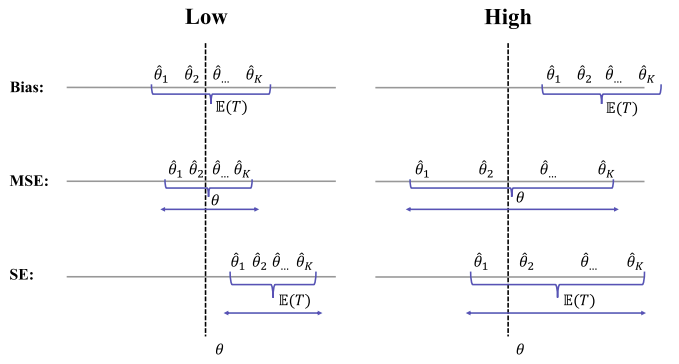
\includegraphics[
        width=0.7\linewidth,
        height=6cm,
        keepaspectratio,
    ]{images/statistics/bias-se-mse-visual.png}
    \caption{Visual Representation of Bias, MSE and SE}
\end{figure}


\subsection{Bias}\label{Sampling Plans/Measures of closeness/Bias}

\hfill
$
    bias
    = \dParenBrac{\dsum_{k=1}^{K} \hat{\theta}_k \pi_k} - \theta
    = \mathbb{E}(T) - \theta
$
\hfill \cite{statistics/book/Statistics-for-Data-Scientists/Maurits-Kaptein}

\vspace{0.5cm}

\begin{enumerate}
    \item The bias is the difference between the weighted average - over all possible $K$ samples - of the sample estimate $\hat{\theta}_k$'s and the true population parameter $\theta$.
    \hfill \cite{statistics/book/Statistics-for-Data-Scientists/Maurits-Kaptein}

    \item The weights in this weighted average are provided by the probabilities $\pi_k$.
    \hfill \cite{statistics/book/Statistics-for-Data-Scientists/Maurits-Kaptein}

    \item  If the bias of an estimator is \textbf{zero}, this means that, if we repeatedly take samples using our sampling plan and repeatedly compute our statistic of interest, the average over all of those statistics is equal to the true population parameter.
    \hfill \cite{statistics/book/Statistics-for-Data-Scientists/Maurits-Kaptein}
    \\
    If the bias is \textbf{zero}, the estimator, under the sampling plan that is being evaluated, is said to be \textbf{unbiased}.
    \hfill \cite{statistics/book/Statistics-for-Data-Scientists/Maurits-Kaptein}

    \item The bias of an estimator is thus the difference between this estimator’s expected value and the true population value.
    \hfill \cite{statistics/book/Statistics-for-Data-Scientists/Maurits-Kaptein}

    \item A small bias of an estimator under a sampling plan does \textbf{not} guarantee that individual sample results $\hat{\theta}_k$ are actually close to the population parameter $\theta$; it just states that they are close on average, if we were to sample over and over again.
    \hfill \cite{statistics/book/Statistics-for-Data-Scientists/Maurits-Kaptein}

    \item If the bias is small, $\mathbb{E}(T)$ is close to the parameter value $\theta$.\\
    If the bias is large, $\mathbb{E}(T)$ is \textbf{not} close to $\theta$
    \hfill \cite{statistics/book/Statistics-for-Data-Scientists/Maurits-Kaptein}

    \item If the sampling plan is unbiased and thus $\mathbb{E}(T) = \theta$, the RMSE and the SE are identical.
    \hfill \cite{statistics/book/Statistics-for-Data-Scientists/Maurits-Kaptein}


\end{enumerate}









\subsection{Mean Square Error (MSE)}\label{Sampling Plans/Measures of closeness/Mean Square Error (MSE)}

\hfill
$
    MSE
    = \dsum_{k=1}^{K} \dParenBrac{\hat{\theta}_k - \theta}^2 \pi_k
$
\hfill \cite{statistics/book/Statistics-for-Data-Scientists/Maurits-Kaptein}


\begin{enumerate}
    \item To capture the variability in the sample results $\hat{\theta}_1, \hat{\theta}_2,..., \hat{\theta}_K$ with respect to the true value $\theta$, we use the so-called mean squared error (MSE).
    \hfill \cite{statistics/book/Statistics-for-Data-Scientists/Maurits-Kaptein}

    \item The MSE measures the weighted average squared distance of the sample results $\hat{\theta}_1, \hat{\theta}_2,..., \hat{\theta}_K$ from the population parameter $\theta$.
    \hfill \cite{statistics/book/Statistics-for-Data-Scientists/Maurits-Kaptein}

    \item The weights are determined by the sampling probabilities.
    \hfill \cite{statistics/book/Statistics-for-Data-Scientists/Maurits-Kaptein}

    \item The smaller the MSE the better the sampling plan.
    \hfill \cite{statistics/book/Statistics-for-Data-Scientists/Maurits-Kaptein}

    \item If the MSE is small, the variability of the $\hat{\theta}_k$'s around $\theta$ is small, \\
    while if the MSE is large, the variability around $\theta$ is large.
    \hfill \cite{statistics/book/Statistics-for-Data-Scientists/Maurits-Kaptein}
\end{enumerate}







\subsection{Root Mean Square Error (RMSE)}\label{Sampling Plans/Measures of closeness/Root Mean Square Error (RMSE)}


\hfill
$
    RMSE
    = \sqrt{MSE}
    = \sqrt{{SE}^2 + \dParenBrac{\mathbb{E}(T) - \theta}^2}
$
\hfill \cite{statistics/book/Statistics-for-Data-Scientists/Maurits-Kaptein}






\subsection{Standard Error (SE)}\label{Sampling Plans/Measures of closeness/Standard Error (SE)}


\hfill
$
    SE = \sqrt{
        \dsum_{k=1}^{K} \dParenBrac{
            \hat{\theta}_k - \mathbb{E}(T)
        }^2
        \pi_k
    }
$
\hfill \cite{statistics/book/Statistics-for-Data-Scientists/Maurits-Kaptein}


\begin{enumerate}
    \item It represents the variability of the sampling plan with respect to the expected population parameter $\mathbb{E}(T)$ instead of using the true population parameter $\theta$.
    \hfill \cite{statistics/book/Statistics-for-Data-Scientists/Maurits-Kaptein}

    \item Standard error of an estimator is used as a measure to represent our uncertainty regarding an estimate.
    \hfill \cite{statistics/book/Statistics-for-Data-Scientists/Maurits-Kaptein}

    \item If the SE is small, the variability of the $\hat{\theta}_k$’s around $\mathbb{E}(T)$ is small.
    \hfill \cite{statistics/book/Statistics-for-Data-Scientists/Maurits-Kaptein}

    \item $SE(cT ) = c\ SE(T) \hspace{2cm} \forall\  c \in \mbbR$
    \hfill \cite{statistics/book/Statistics-for-Data-Scientists/Maurits-Kaptein}
\end{enumerate}








\section{Types of Samplings}

\begin{enumerate}

\item \textbf{Non-representative Sampling} \label{Sampling Plans/Non-representative Sampling}
\hfill \cite{statistics/book/Statistics-for-Data-Scientists/Maurits-Kaptein}

    \begin{enumerate}
        \item Although these sampling methods are frequently in use, it is strongly recommended not to apply these methods, unless knowledge is available on how to adjust or correct the sample for inferential purposes.
        \hfill \cite{statistics/book/Statistics-for-Data-Scientists/Maurits-Kaptein}

        \item These have the risk that some units are much more likely to be included in the sample than others, which can make statistics computed on the sample data bad estimates for the population parameters of interest.
        \hfill \cite{statistics/book/Statistics-for-Data-Scientists/Maurits-Kaptein}

        \item With non-representative sampling some units are not only more likely to be included in the sample, we also do not actually know how likely units were included.
        \hfill \cite{statistics/book/Statistics-for-Data-Scientists/Maurits-Kaptein}

        \item Even if we wanted to, we could not control for these systematic differences between units.
        \hfill \cite{statistics/book/Statistics-for-Data-Scientists/Maurits-Kaptein}
    \end{enumerate}

    \vspace{0.2cm}
    \textbf{SEE}:
    \begin{enumerate}
        \item \fullref{Sampling Plans/Non-representative Sampling/Convenience Sampling}
        \item \fullref{Sampling Plans/Non-representative Sampling/Haphazard Sampling}
        \item \fullref{Sampling Plans/Non-representative Sampling/Purposive Sampling or Judgmental Sampling}
    \end{enumerate}


\item \textbf{Representative Sampling} \label{Sampling Plans/Representative Sampling}
\hfill \cite{statistics/book/Statistics-for-Data-Scientists/Maurits-Kaptein}
    \begin{enumerate}
        \item We sample units in such a way that we do know how likely units are to be included in the sample (even if they will be different from unit to unit).
        \hfill \cite{statistics/book/Statistics-for-Data-Scientists/Maurits-Kaptein}

        \item Random sampling is a sampling method that uses a random mechanism.
        \hfill \cite{statistics/book/Statistics-for-Data-Scientists/Maurits-Kaptein}

        \begin{enumerate}
            \item The probability of each unit in the population of becoming part of the sample is both positive and known.
            \hfill \cite{statistics/book/Statistics-for-Data-Scientists/Maurits-Kaptein}
        \end{enumerate}
    \end{enumerate}

    \vspace{0.2cm}
    \textbf{SEE}:
    \begin{enumerate}
        \item \fullref{Sampling Plans/Representative Sampling/Simple Random Sampling}
        \item \fullref{Sampling Plans/Representative Sampling/Systematic Sampling}
        \item \fullref{Sampling Plans/Representative Sampling/Stratified Sampling}
        \item \fullref{Sampling Plans/Representative Sampling/Cluster Sampling}
    \end{enumerate}
\end{enumerate}

\clearpage
\section{Convenience Sampling \cite{statistics/book/Statistics-for-Data-Scientists/Maurits-Kaptein}}\label{Sampling Plans/Non-representative Sampling/Convenience Sampling}

\begin{enumerate}
    \item Convenience sampling collects only units from the population that can be easily obtained.
    \hfill \cite{statistics/book/Statistics-for-Data-Scientists/Maurits-Kaptein}

    \item This may provide a biased sample, as it represents only one small part or time window of the whole processing window for a batch of products. The term \textbf{bias}\label{Sampling Plans/Non-representative Sampling/Convenience Sampling/bias} indicates that we obtain the value of interest with a systematic mistake.
    \hfill \cite{statistics/book/Statistics-for-Data-Scientists/Maurits-Kaptein}

    \item  Convenience sampling is often justified by using the argument of population homogeneity. This insinuates that either the population units are not truly different or the process produces the population of units in random order. 
    \hfill \cite{statistics/book/Statistics-for-Data-Scientists/Maurits-Kaptein}
\end{enumerate}


\section{Haphazard Sampling \cite{statistics/book/Statistics-for-Data-Scientists/Maurits-Kaptein}}\label{Sampling Plans/Non-representative Sampling/Haphazard Sampling}

\begin{enumerate}
    \item Haphazard sampling is often believed to be an excellent way of collecting samples, because it gives a feeling or the impression that each unit was collected completely at random.
    \hfill \cite{statistics/book/Statistics-for-Data-Scientists/Maurits-Kaptein}

    \item Despite the feeling of randomness when performing haphazard sampling, often the resulting sample is not truly random.
    \hfill \cite{statistics/book/Statistics-for-Data-Scientists/Maurits-Kaptein}
\end{enumerate}

\section{Purposive Sampling/ Judgmental Sampling \cite{statistics/book/Statistics-for-Data-Scientists/Maurits-Kaptein}}\label{Sampling Plans/Non-representative Sampling/Purposive Sampling or Judgmental Sampling}

\begin{enumerate}
    \item Purposive sampling or judgmental sampling tries to sample units for a specific purpose.
    \hfill \cite{statistics/book/Statistics-for-Data-Scientists/Maurits-Kaptein}

    \item This means that the collection of units is focused on one or more particular characteristics and hence it implies that only units that are more alike are sampled.
    \hfill \cite{statistics/book/Statistics-for-Data-Scientists/Maurits-Kaptein}

    \item This way of sampling is strongly related to the definition of the population, since deliberately excluding units from the sample is analogous to limiting the population of interest.
    \hfill \cite{statistics/book/Statistics-for-Data-Scientists/Maurits-Kaptein}

    \item Purposive sampling may be useful, but it is limited since it does not allow us in general to make statements about the whole population, and at best only about a limited part of the population (although we may not be sure either).
    \hfill \cite{statistics/book/Statistics-for-Data-Scientists/Maurits-Kaptein}

    \item It does most likely produce a biased sample with respect to the complete population.
    \hfill \cite{statistics/book/Statistics-for-Data-Scientists/Maurits-Kaptein}
\end{enumerate}


\clearpage
\section{Simple Random Sampling \cite{statistics/book/Statistics-for-Data-Scientists/Maurits-Kaptein}}\label{Sampling Plans/Representative Sampling/Simple Random Sampling}

\begin{table}[H]
    \centering
    \begin{tabular}{l l}
        $N$ & population size \\
        $n$ & sample size \\
        $K$ & number of possible samples \\
        $k$ & sample index ($ k \in \dParenBrac{1,\cdots,K}$) \\
        $S_k$ & sample\\
    \end{tabular}
\end{table}

\begin{enumerate}
    \item Implicitly assume that there is no particular group structure present in the population.
    \hfill \cite{statistics/book/Statistics-for-Data-Scientists/Maurits-Kaptein}

    \item Simple random sampling is a way of collecting samples such that each unit from the population has the exact same probability of becoming part of the sample.
    \hfill \cite{statistics/book/Statistics-for-Data-Scientists/Maurits-Kaptein}


    \item Simple random sampling is a conceptually easy method of forming random samples but it can prove hard in practice.
    \hfill \cite{statistics/book/Statistics-for-Data-Scientists/Maurits-Kaptein}

    \item Simple random sampling is frequently combined with other choices or settings (see stratified and cluster sampling).
    \hfill \cite{statistics/book/Statistics-for-Data-Scientists/Maurits-Kaptein}

    \item Number of unique samples $
        = K
        = \dfrac{N!}{n!(N-n)!}
    $
    \hfill \cite{statistics/book/Statistics-for-Data-Scientists/Maurits-Kaptein}

    \item the probability of collecting sample $S_k$, using sequential sampling $
        = \dfrac{1}{K}
        = \dfrac{n!(N-n)!}{N!}
    $
    \hfill \cite{statistics/book/Statistics-for-Data-Scientists/Maurits-Kaptein}

    \item The probability that a specific unit is part of the sample $
        = \dfrac{n}{N}
    $
    \hfill \cite{statistics/book/Statistics-for-Data-Scientists/Maurits-Kaptein}

    \item The probability that a specific unit is \textbf{not} contained in the sample $
        = 1 - \dfrac{n}{N}
        = \dfrac{N-n}{N}
    $
    \hfill \cite{statistics/book/Statistics-for-Data-Scientists/Maurits-Kaptein}

    \item The number of samples that does \textbf{not} contain a specific unit $
        = \dfrac{(N - 1)!}{n!(N - 1 - n)!}
    $
    \hfill \cite{statistics/book/Statistics-for-Data-Scientists/Maurits-Kaptein}

    \item Number of samples that contain certain unit $i$ = $\dfrac{nK}{N}$
    \hfill \cite{statistics/book/Statistics-for-Data-Scientists/Maurits-Kaptein}
    \\
    $
        \Rightarrow
        \dsum_{k=1}^{K}\ \dsum_{i \in S_k} x_i
        = \dfrac{nK}{N}\dsum_{i=1}^{N} x_i
    $
    \hfill \cite{statistics/book/Statistics-for-Data-Scientists/Maurits-Kaptein}

    \item Population Variance: $
        \sigma^2
        = \dfrac{1}{N} \dsum_{i=1}^N (x_i-\mu)^2
    $
    \hfill \cite{statistics/book/Statistics-for-Data-Scientists/Maurits-Kaptein}

    \item \textbf{Disadvantage}: When the numbers of units across these subpopulations are (substantially) different, simple random may not collect units from each subgroup.
    \hfill \cite{statistics/book/Statistics-for-Data-Scientists/Maurits-Kaptein}

\end{enumerate}

\vspace{0.5cm}
\textbf{Example}:
\begin{enumerate}
    \item[] $N = 20,\ n = 5$

    \item[] $K = \dfrac{20!}{5!\cdot 15!}=15504$


\end{enumerate}


\subsection{Estimation for population mean}
\begin{enumerate}
    \item Estimator: $
        T
        = \bar{x}
        = \dfrac{1}{n} \dsum_{i=1}^n x_i
    $
    \hfill \cite{statistics/book/Statistics-for-Data-Scientists/Maurits-Kaptein}

    \item Bias: $0$
    \hfill \cite{statistics/book/Statistics-for-Data-Scientists/Maurits-Kaptein}

    \item $
        MSE(\bar{x}_k)
        = \dfrac{\sigma^2 }{n}
        \dParenBrac{\dfrac{N}{N-1}}
        \dParenBrac{1-\dfrac{n}{N}}
        = \dfrac{\sigma^2\ (N-n)}{n\ (N-1)}
    $
    \hfill \cite{statistics/book/Statistics-for-Data-Scientists/Maurits-Kaptein}
    \\
    MSE shows that it becomes equal to zero when the sample size $n$ becomes equal to the population size $N$.
    \hfill \cite{statistics/book/Statistics-for-Data-Scientists/Maurits-Kaptein}
    \\
    The MSE will not become zero when the estimator is biased, even if the sample size is equal to the population size.
    \hfill \cite{statistics/book/Statistics-for-Data-Scientists/Maurits-Kaptein}


    \item $
        \mathbb{E}[T]
        = \dfrac{1}{K}\dsum_{k=1}^{K} \bar{x}_k
        = \dfrac{1}{nK}\dsum_{k=1}^{K}\ \dsum_{i \in S_k} x_i
        = \dfrac{1}{N}\dsum_{i=1}^{N} x_i
        = \mu
    $
    \hfill \cite{statistics/book/Statistics-for-Data-Scientists/Maurits-Kaptein}
\end{enumerate}


\subsection{Estimation of the sample MSE}

\begin{enumerate}
    \item unbiased estimator for $\sigma^2$: \\
    $
       \hat{\sigma}^2 = \dfrac{N - 1}{N}\ s^2_k
    $
    \hfill
    $
        \dParenBrac{\
            s^2_k = \dfrac{1}{n - 1} \dsum_{i\ \in\ S_k} (x_i - \bar{x}_k )^2
        \ }
    $
    \hfill \cite{statistics/book/Statistics-for-Data-Scientists/Maurits-Kaptein}

    \item $
        \hat{MSE}(\bar{x}_k)
        = \dfrac{N - n}{N n}\ s^2_k
    $
    \hfill \cite{statistics/book/Statistics-for-Data-Scientists/Maurits-Kaptein}

    \item This is an unbiased estimator of the MSE of the arithmetic average in $MSE(\bar{x}_k)$ and it may also be used when the observations are binary.
    \hfill \cite{statistics/book/Statistics-for-Data-Scientists/Maurits-Kaptein}


\end{enumerate}




\subsection{Sample Statistics ($T_n$)}

\begin{enumerate}
    \item We can view a sample $X_1 , X_2 , \cdots, X _n$ of size $n$ from a population as a set of random variables (and $x_1 , x_2, \cdots , x _n$ as the set of realizations) all coming from the same distribution function $F$.
    Let $X_1 , X_2, \cdots , X _n$ be i.i.d. with $X _i \sim F$
    \hfill \cite{statistics/book/Statistics-for-Data-Scientists/Maurits-Kaptein}

    \item A sample statistic $T_n \in \mbbR$ is now defined as any function $T_n \equiv T (X_1, X_2, \cdots , X _n )$ that is applied to the sample $X_1 , X_2, \cdots , X _n$.
    As $T_n$ is a function of random variables, it is itself a random variable.
    \hfill \cite{statistics/book/Statistics-for-Data-Scientists/Maurits-Kaptein}

    \item realization for the sample statistic $T_n$: $t _n = T (x_1, x_2, \cdots , x _n )$
    \hfill \cite{statistics/book/Statistics-for-Data-Scientists/Maurits-Kaptein}

    \item \textbf{Sample average}: $T_n = \bar{X} = \dfrac{1}{n}\dsum^n _{i=1} X _i$
    \hfill \cite{statistics/book/Statistics-for-Data-Scientists/Maurits-Kaptein}

    \item \textbf{Sample variance}: $T_n = S^2 = \dfrac{1}{n - 1} \dsum^n _{i=1}(X _i - \bar{X})^2$
    \hfill \cite{statistics/book/Statistics-for-Data-Scientists/Maurits-Kaptein}

    \item \textbf{Sample standard deviation}: $T_n = S^2 = \sqrt{\dfrac{1}{n - 1} \dsum^n _{i=1}(X _i - \bar{X})^2}$
    \hfill \cite{statistics/book/Statistics-for-Data-Scientists/Maurits-Kaptein}

    \item \textbf{Sample skewness}: $T_n = b_1 = \dfrac{1}{n S^3} \dsum^n _{i=1} (X _i - \bar{X})^3$
    \hfill \cite{statistics/book/Statistics-for-Data-Scientists/Maurits-Kaptein}

    \item \textbf{Sample excess kurtosis}: $T_n = b_2 = \dParenBrac{\dfrac{1}{n S^4} \dsum^n _{i=1} (X _i - \bar{X})^4} - 3$
    \hfill \cite{statistics/book/Statistics-for-Data-Scientists/Maurits-Kaptein}

    \item \textbf{Sample minimum}: $T_n = X_{(1)} = \min \dCurlyBrac{X_1, X_2, \cdots, X _n }$
    \hfill \cite{statistics/book/Statistics-for-Data-Scientists/Maurits-Kaptein}

    \item \textbf{Sample maximum}: $T_n = X_{(n)} = \max \dCurlyBrac{X_1, X_2, \cdots, X _n }$
    \hfill \cite{statistics/book/Statistics-for-Data-Scientists/Maurits-Kaptein}

    \item \textbf{quantile}:
    \begin{enumerate}
        \item If $np \in \mathbb{N}$ is an integer, the quantile $x _p$ is estimated by the average of two sequential order statistics: $q _p = \dfrac{[X_{(np)} + X_{(1+np)}]}{2}$.
        \hfill \cite{statistics/book/Statistics-for-Data-Scientists/Maurits-Kaptein}

        \item If $np \notin \mathbb{N}$ is not an integer, we take the smallest integer value that is larger than or equal to $np$, which is denoted by $\dceil{np}$.
        \hfill \cite{statistics/book/Statistics-for-Data-Scientists/Maurits-Kaptein}
    \end{enumerate}
\end{enumerate}




\clearpage
\section{Systematic Sampling \cite{statistics/book/Statistics-for-Data-Scientists/Maurits-Kaptein}}\label{Sampling Plans/Representative Sampling/Systematic Sampling}

\begin{table}[H]
    \centering
    \begin{tabular}{l l l}
        $N$ & population size & $N=nm$\\
        $n$ & number of groups & = sample size \\
        $m$ & number of units in each group & = number of possible samples\\
        $k$ & sample index & $k \in \dParenBrac{1,\cdots,m}$ \\
        $S_k$ & sample & \\
    \end{tabular}
\end{table}

\begin{enumerate}
    \item Implicitly assume that there is no particular group structure present in the population.
    \hfill \cite{statistics/book/Statistics-for-Data-Scientists/Maurits-Kaptein}

    \item Steps:
    \hfill \cite{statistics/book/Statistics-for-Data-Scientists/Maurits-Kaptein}
    \begin{enumerate}
        \item First the population should be divided into $n$ groups and the order of the units (if Some order exists) should be maintained (or otherwise fix the order).\\
        Each group consists of $m$ units ordered from $1$ to $m$ in each group.

        \item Collect $p$th unit ($p \in \dParenBrac{1,\cdots,m}$) from all $n$ groups with probability of $\dfrac{1}{m}$\\
        (each unit in the population still has the same probability of being collected)\\
        $S_k = \dCurlyBrac{k, k + m, k + 2m, \cdots , k + (n - 1)m}$ 
        \hfill
        (Total units collected $= n$) 
        \hfill \cite{statistics/book/Statistics-for-Data-Scientists/Maurits-Kaptein} \\
        So, total number of samples $= m$ only

    \end{enumerate}

    \item The possible samples from systematic sampling are quite different from the set of samples that can be obtained with simple random sampling.
    \hfill \cite{statistics/book/Statistics-for-Data-Scientists/Maurits-Kaptein}

    \item population mean: $
        \mu 
        = \dfrac{1}{N}\ \dsum^m_{h=1} \ \dsum^n_{i=1} x_{\ k+m(i-1)}
    $
    \hfill \cite{statistics/book/Statistics-for-Data-Scientists/Maurits-Kaptein}

    \item population variance: $
        \sigma^2 
        = \dfrac{1}{N}\ \dsum^m_{k=1} \ \dsum^n_{i=1} (x_{\ k+m(i-1)} - \mu)^2
    $
    \hfill \cite{statistics/book/Statistics-for-Data-Scientists/Maurits-Kaptein}
    
    \item sample average for sample $S_k$: $
        \bar{x}_k 
        = \dfrac{1}{n}\ \dsum^n_{i=1} x_{\ k+m(i-1)}
    $
    \hfill \cite{statistics/book/Statistics-for-Data-Scientists/Maurits-Kaptein}

    \item Systematic sampling can be more efficient than simple random sampling, in particular when the variance in the systematic samples is larger than the population variance (which is impossible to verify in practice).
    \hfill \cite{statistics/book/Statistics-for-Data-Scientists/Maurits-Kaptein}

    \item The most important \textbf{advantage} of systematic sampling over simple random sampling is the ease with which the sample may be collected.
    \hfill \cite{statistics/book/Statistics-for-Data-Scientists/Maurits-Kaptein}

    \item A clear \textbf{disadvantage} of systematic sampling is that the “period” for systematic sampling may coincide with particular patterns in the process or population.
    \hfill \cite{statistics/book/Statistics-for-Data-Scientists/Maurits-Kaptein}

    \item \textbf{Disadvantage}: When the numbers of units across these subpopulations are (substantially) different, systematic sampling may not collect units from each subgroup.
    \hfill \cite{statistics/book/Statistics-for-Data-Scientists/Maurits-Kaptein}

    \item TODO? Systematic Sampling samples ($S_1,\cdots,S_m$) are subset of Simple Random Sampling samples ($S_1,\cdots,S_K$).
\end{enumerate}

\vspace{0.5cm}
\textbf{Example}:
\begin{enumerate}
    \item[] $N = 20,\ n = 5$

    \item[] $m = \dfrac{20}{5}=4$

    
\end{enumerate}



\subsection{Estimation for population mean}
\begin{enumerate}
    \item Estimator: $
        \dfrac{1}{n} \dsum_{i=1}^n x_i
    $
    \hfill \cite{statistics/book/Statistics-for-Data-Scientists/Maurits-Kaptein}
    \\
    if population can be perfectly split up into $n$ groups of $m$ units:\\
    Unbiased Estimator: $\bar{x}_k$
    
    \item Bias: $0$
    \hfill \cite{statistics/book/Statistics-for-Data-Scientists/Maurits-Kaptein}

    \item MSE: $
        \sigma^2 -
        \dfrac{1}{N}
        \dsum_{h=1}^{n}
        \dsum_{i=1}^{m}
        (x_{h+m(i-1)} - \bar{x}_h)^2
    $
    \hfill \cite{statistics/book/Statistics-for-Data-Scientists/Maurits-Kaptein}

\end{enumerate}



\subsection{Estimation of the MSE}

\begin{enumerate}
    \item In the general setting for systematic sampling, an unbiased estimation of the MSE is \textbf{not possible}.
    \hfill \cite{statistics/book/Statistics-for-Data-Scientists/Maurits-Kaptein}

    \item Given that there is no systematic difference between units based on their position in the groups (and the ratio of sample and population size is an integer), the MSE of the sample average under systematic sampling becomes equal to the MSE of the sample average under simple random sampling.
    \hfill \cite{statistics/book/Statistics-for-Data-Scientists/Maurits-Kaptein}
    
    \item unbiased estimator: $
        \dfrac{N - 1}{N}\ s^2_k
    $
    \hfill
    $
        s^2_k = \dfrac{1}{n - 1} \dsum^n_{i=1} (x_{k+m(i-1)} - \bar{x}_k )^2
    $
    \hfill \cite{statistics/book/Statistics-for-Data-Scientists/Maurits-Kaptein}
\end{enumerate}






\clearpage
\section{Stratified Sampling \cite{statistics/book/Statistics-for-Data-Scientists/Maurits-Kaptein}}\label{Sampling Plans/Representative Sampling/Stratified Sampling}

\begin{customArrayStretch}{1.3}
\begin{longtable}{>{\centering\arraybackslash}p{1.5cm} p{9cm} p{3.5cm}}

\hline\endfirsthead
\hline\endhead
\hline\endfoot
\hline\endlastfoot

$N$ & total population size & \\ \hline

$n$ & total sample size & \\ \hline

$M$ & number of sub-populations & \\ \hline

$N_h$ & $k$th sub-population size & $\tsum_{h=1}^{M} N_h = N$ \\ \hline

$n_h$ & sample size from $k$th sub-population & $\tsum_{h=1}^{M} n_h = n$ \\ \hline

$h$ & Stratum index & $h \in \dCurlyBrac{1, \cdots, M}$ \\ \hline

$k$ & Stratum index & $k \in \dCurlyBrac{1, \cdots, K_S}$ \\ \hline

$K_h$ & The number of possible samples that can be drawn from stratum $h$ \\ \hline

$K_S$ & total number of possible samples \\ \hline

$(h, i)$ & index of unit & \begin{minipage}{3.2cm}
    \vspace{0.1cm}
    $i \in \dCurlyBrac{1, 2,\cdots, N_h }$ \\
    and $h \in \dCurlyBrac{1, 2,..., M}$
    \vspace{0.1cm}
\end{minipage}  \\ \hline

$x_{hi}$ & unit $i$ in stratum $h$ \\ \hline

$w_{h}$ &
    weight of strata $h$ while sampling &
    \begin{minipage}{3.2cm}
        \vspace{0.1cm}
        $w_{h} = \dfrac{N_h}{N}$
        \vspace{0.1cm}
    \end{minipage}
    \\ \hline

$f_{h}$ &
    sample fraction in stratum $h$ &
    \begin{minipage}{3.2cm}
        \vspace{0.1cm}
        $f_{h} = \dfrac{n_h}{N_h}$
        \vspace{0.1cm}
    \end{minipage}
    \\ \hline

$S_{h,k}$ &
\multicolumn{2}{l}{
    \begin{minipage}{11cm}
        \vspace{0.1cm}
        $S_{h,k}$ is the collected sample in stratum $h$ \\
        The $k$-th possible sample from stratum $h$ \\
        (e.g., $S_{2,3}$ is the $3$rd possible sample from stratum $2$) \\
        focuses on one stratum
        \vspace{0.1cm}
    \end{minipage}
} \\ \hline

$S_k$ &
\multicolumn{2}{l}{
    \begin{minipage}{11cm}
        \vspace{0.1cm}
        The $k$-th possible full stratified sample (i.e., across all strata). \\
        Each $S_k$ includes one selected sample from each stratum.\\
        focuses on a complete sample (all strata combined)
        \vspace{0.1cm}
    \end{minipage}
} \\ \hline

\end{longtable}
\end{customArrayStretch}

\begin{enumerate}
    \item Stratified sampling is used to accommodate the issue of missing out on sub-populations during sampling by setting the sample size for each subpopulation (often called \textbf{strata}\label{Sampling Plans/Representative Sampling/Stratified Sampling/strata}) to a fixed percentage of the number of units of the subpopulation.
    \hfill \cite{statistics/book/Statistics-for-Data-Scientists/Maurits-Kaptein}

    \item Steps:
    \hfill \cite{statistics/book/Statistics-for-Data-Scientists/Maurits-Kaptein}
    \begin{enumerate}
        \item The population is then divided into $n$ groups such that the order in units is maintained.

        \item From $k$th group/ strata one unit is randomly collected with probability $\dfrac{n_h}{N_h}$, when each group contains $n_h$ units.\\
        Unlike systematic sampling, random unit is collected instead of $p$th unit.
    \end{enumerate}

    \item This form of stratified sampling is not identical to systematic sampling (although this method of stratified sampling is sometimes referred to as systematic sampling).
    \hfill \cite{statistics/book/Statistics-for-Data-Scientists/Maurits-Kaptein}

    \item Stratified sampling may lead to samples that are not possible with systematic sampling, but it does not produce all possible samples from simple random sampling.
    \hfill \cite{statistics/book/Statistics-for-Data-Scientists/Maurits-Kaptein}

    \item $
        K_h = \binom{N_h}{n_h} = \dfrac{N_h!}{n_h!(N_h-n_h)!}
    $
    \hfill \cite{statistics/book/Statistics-for-Data-Scientists/Maurits-Kaptein}

    \item The number of possible samples: $
        K_S
        = \dprod_{h=1}^{M} \dfrac{N_h!}{n_h!(N_h-n_h)!}
        = \dprod_{h=1}^{M} K_h
    $
    \hfill \cite{statistics/book/Statistics-for-Data-Scientists/Maurits-Kaptein}

    \item The probability of collecting any of the $K_S$ samples $
        = \dfrac{1}{K_S}
    $
    \hfill \cite{statistics/book/Statistics-for-Data-Scientists/Maurits-Kaptein}

    \item The probability of collecting a unit now depends on the stratum the unit is part of.
    \hfill \cite{statistics/book/Statistics-for-Data-Scientists/Maurits-Kaptein}

    \item If $
        \dfrac{n_i}{N_i} = \dfrac{n_j}{N_j}
        \hspace{0.3cm}
        \forall
        \hspace{0.3cm}
        i,j \in \dParenBrac{1,\cdots,M}
    $, then its called \textbf{Proportional Stratified Sampling}.\label{Sampling Plans/Representative Sampling/Stratified Sampling/Proportional Stratified Sampling}
    \hfill \cite{statistics/book/Statistics-for-Data-Scientists/Maurits-Kaptein}

\end{enumerate}


\vspace{0.5cm}\hspace{0cm}
\textbf{Example}: sample $10\%$ from each sub-population


\subsection{population stratum}
\begin{enumerate}
    \item population stratum mean: $
        \mu_h = \dfrac{1}{N_h} \ \dsum_{i=1}^{N_h} \ x_{hi}
    $
    \hfill \cite{statistics/book/Statistics-for-Data-Scientists/Maurits-Kaptein}

    \item population stratum variance: $
        \sigma^2_h = \dfrac{1}{N_h} \ \dsum_{i=1}^{N_h} \ (x_{hi} - \mu_h)^2
    $
    \hfill \cite{statistics/book/Statistics-for-Data-Scientists/Maurits-Kaptein}

\end{enumerate}



\subsection{population}
\begin{enumerate}
    \item population mean: $
        \mu
        = \dfrac{1}{N} \ \dsum_{h=1}^M \ \dsum_{i=1}^n\  x_{hi}
        = \dsum_{h=1}^M \ w_h\mu_h
    $
    \hfill \cite{statistics/book/Statistics-for-Data-Scientists/Maurits-Kaptein}
    \begin{enumerate}
        \item $w_h = \dfrac{N_h}{N}$
        \hfill \cite{statistics/book/Statistics-for-Data-Scientists/Maurits-Kaptein}

        \item $\dsum_{h=1}^M \ w_h = 1$
        \hfill \cite{statistics/book/Statistics-for-Data-Scientists/Maurits-Kaptein}
    \end{enumerate}


    \item population variance: $
        \sigma^2
        \equiv \dfrac{1}{N} \ \dsum_{h=1}^M \ \dsum_{i=1}^{N_h} (x_{hi} - \mu)^2
        = \dsum_{h=1}^M w_h \sigma_h^2 + \dsum_{h=1}^M w_h (\mu_h - \mu)^2
    $
    \hfill \cite{statistics/book/Statistics-for-Data-Scientists/Maurits-Kaptein}
    \vspace{0.15cm}
    \begin{enumerate}
        \item \textbf{within (strata) variances}: the first part represents a weighted mean of the within strata variances

        \item \textbf{between (strata) variances}: the second part represents a weighted mean of the squared distances of the strata means to the population mean
    \end{enumerate}

\end{enumerate}


\subsubsection{Estimation for population mean}
\begin{enumerate}
    \item Estimator: $
        \dsum_{h=1}^{M}
        \dfrac{N_h}{N}
        \dParenBrac{\dfrac{1}{n_h} \dsum_{i=1}^{n_h} x_{hi}}
        =
        \dsum_{h=1}^{M} \ w_h \ \bar{x}_{h,k}
    $
    \hfill \cite{statistics/book/Statistics-for-Data-Scientists/Maurits-Kaptein}

    \item Bias: $0$
    \hfill \cite{statistics/book/Statistics-for-Data-Scientists/Maurits-Kaptein}

    \item MSE: $
        \dsum_{h=1}^{M}
        \dSquareBrac{
            \dParenBrac{
                \dfrac{
                    N_h^2\ (N_h - n_h)
                }{
                    n_h\ (N_h-1)\ N^2
                }
            } \sigma_h^2
        }
    $
    \hfill \cite{statistics/book/Statistics-for-Data-Scientists/Maurits-Kaptein}
\end{enumerate}




\subsection{sample stratum}
\begin{enumerate}
    \item sample stratum mean: $
        \bar{x}_{h,k} = \dfrac{1}{n_h} \ \dsum_{i \ \in \ S_{h,k}} \ x_{hi}
    $
    \hfill \cite{statistics/book/Statistics-for-Data-Scientists/Maurits-Kaptein}

    \item sample stratum variance: $
        s^2_{h,k} = \dfrac{1}{n_h-1} \ \dsum_{i \ \in \ S_{h,k}} \ (x_{hi} - \bar{x}_{h,k})^2
    $
    \hfill \cite{statistics/book/Statistics-for-Data-Scientists/Maurits-Kaptein}

    \item MSE for unbiased estimator:
    $
        MSE(\bar{x}_{h,k}) = \tVar[\bar{x}_{h,k}] = SE^2(\bar{x}_{h,k})
    $
    \hfill \cite{common/online/chatgpt}

    \item The bias and standard error within each stratum $h$ now follow the theory of simple random sampling.
    \hfill \cite{statistics/book/Statistics-for-Data-Scientists/Maurits-Kaptein}

    \item bias of $\bar{x}_{h,k}$ = 0 in stratum $h$ is zero for the stratum mean $\mu_h$

\end{enumerate}


\subsubsection{Estimation for sample stratum SE}
\begin{enumerate}
    \item $
        \hat{SE}(\bar{x}_{h,k})
        = \sqrt{\dfrac{1 - f_h}{n_h}} s_{h,k}
    $
    \hfill
    $f_h = \dfrac{n_h}{N_h}$
    \hfill \cite{statistics/book/Statistics-for-Data-Scientists/Maurits-Kaptein}
\end{enumerate}



\subsection{sample}
\begin{enumerate}
    \item Sample average: $
        \bar{x}_k = \dsum^M_{h=1} w_h\ \bar{x}_{h,k}
    $
    \hfill \cite{statistics/book/Statistics-for-Data-Scientists/Maurits-Kaptein}

    \item the \textit{simple random samples} from the different strata are completely \textbf{unrelated}, which implies that the sum of the squared standard errors of $w_h \ \bar{x}_{h,k}$ form the squared standard error of the sample average $\bar{x}_k$.
    \hfill \cite{statistics/book/Statistics-for-Data-Scientists/Maurits-Kaptein}
    \\
    $
        \tVar[\bar{x}_k] = \dsum_{h=1}^M w_h^2 \cdot \tVar[\bar{x}_{h,k}]
    $
    \hfill \cite{common/online/chatgpt}


    \item squared standard error of $\bar{x}_k$:
    $
        SE^2(\bar{x}_k) = \dsum_{h=1}^M w_h^2 \cdot SE^2(\bar{x}_{h,k})
    $
    \hfill \cite{common/online/chatgpt}

    \item $
        MSE(\bar{x}_k )
        = \dsum^M_{h=1} w^2_h \cdot MSE(\bar{x}_{h,k} )
        = \dsum^M_{h=1} \dfrac{N_h}{(N_h - 1)n_h} \ (1 - f_h)\ w^2_h\ \sigma^2_h$
    \hfill \cite{statistics/book/Statistics-for-Data-Scientists/Maurits-Kaptein}

\end{enumerate}


\subsubsection{Estimation of the sample MSE}

$
    \hat{MSE} (\bar{x}_k )
    = \dsum^M_{h=1} \dfrac{1 - f_h}{n_h} \ w^2_h\ s^2_{h,k}.
$
\hfill \cite{statistics/book/Statistics-for-Data-Scientists/Maurits-Kaptein}

SEE: \url{https://chatgpt.com/share/680251af-c100-800a-a533-c26a0001b651}

\subsubsection{Estimation of the sample SE}

An estimate of the standard error of $\bar{x}_k$ is now obtained by taking the square root of
the estimated MSE:
\hfill \cite{statistics/book/Statistics-for-Data-Scientists/Maurits-Kaptein}
\\
$
    \hat{SE}(\bar{x}_k) = \sqrt{\hat{MSE} (\bar{x}_k )}
$














\clearpage
\section{Cluster Sampling \cite{statistics/book/Statistics-for-Data-Scientists/Maurits-Kaptein}}\label{Sampling Plans/Representative Sampling/Cluster Sampling}

\begin{enumerate}[itemsep=0.2cm]
    \item Cluster sampling involves random sampling of groups or clusters of units in the population.
    \hfill \cite{statistics/book/Statistics-for-Data-Scientists/Maurits-Kaptein}

    \item Cluster sampling can be less representative than sampling units directly.
    \hfill \cite{statistics/book/Statistics-for-Data-Scientists/Maurits-Kaptein}

    \item Cluster sampling introduces a specific structure in the sample which should also be addressed when the data is being analyzed. 
    \hfill \cite{statistics/book/Statistics-for-Data-Scientists/Maurits-Kaptein}
    
    \item The cluster structure introduces two sources of variation in the data being collected. These sources of variation need to be quantified to make proper statements on the population of interest.
    \hfill \cite{statistics/book/Statistics-for-Data-Scientists/Maurits-Kaptein}
    \begin{enumerate}[itemsep=0.1cm]
        \item \textbf{Within-Cluster Variation}:\label{Sampling Plans/Representative Sampling/Cluster Sampling/Within-Cluster Variation}
        \hfill \cite{common/online/chatgpt}
        \begin{enumerate}
            \item This refers to the differences among units within the same cluster.
            \hfill \cite{common/online/chatgpt}

            \item This variation is often smaller compared to between-cluster variation because individuals within a cluster tend to be more similar.
            \hfill \cite{common/online/chatgpt}

        \end{enumerate}

        \item \textbf{Between-Cluster Variation}:\label{Sampling Plans/Representative Sampling/Cluster Sampling/Between-Cluster Variation}
        \hfill \cite{common/online/chatgpt}
        \begin{enumerate}
            \item This refers to the differences between clusters.
            \hfill \cite{common/online/chatgpt}

            \item This variation is often larger in cluster sampling because different clusters may have distinct characteristics.
            \hfill \cite{common/online/chatgpt}

        \end{enumerate}
        
    \end{enumerate}

    \item The sampling units for the \textit{first stage} are referred to as \textbf{primary cluster units}\label{Sampling Plans/Representative Sampling/Cluster Sampling/primary cluster units}.
    \hfill \cite{statistics/book/Statistics-for-Data-Scientists/Maurits-Kaptein}

    \item Sampling these different levels of clusters can be performed using simple random sampling, systematic sampling, or even stratified sampling, if certain cluster are put together on certain criteria.
    \hfill \cite{statistics/book/Statistics-for-Data-Scientists/Maurits-Kaptein}

    \item Cluster sampling is in a way related to stratified sampling (clusters may be viewed as strata).
    \hfill \cite{statistics/book/Statistics-for-Data-Scientists/Maurits-Kaptein}

    \item Since we deal with multiple levels of hierarchical clusters, the calculation of the probability of collecting one unit from the population and the probability of collecting one of the many sample sets are complex.
    \hfill \cite{statistics/book/Statistics-for-Data-Scientists/Maurits-Kaptein}
\end{enumerate}




\subsection{Single-Stage Cluster Sampling}\label{Sampling Plans/Representative Sampling/Cluster Sampling/Single-Stage Cluster Sampling}

A single-stage cluster sample uses a random sample of the clusters and then all units from these clusters are selected. 
\hfill \cite{statistics/book/Statistics-for-Data-Scientists/Maurits-Kaptein}

\subsubsection{cluster sizes are not all equal}
    
Estimator for population mean: $
    \dsum_{h=1}^{m}
    \dParenBrac{
        \dfrac{N_h}{
            \tsum_{h=1}^{m} N_h
        }
    }
    \bar{x}_h
$
\hfill \cite{statistics/book/Statistics-for-Data-Scientists/Maurits-Kaptein}

\begin{enumerate}[itemsep=0.25cm]
    \item Bias: $\geq 0$ (bias is close to zero but positive)
    \hfill \cite{statistics/book/Statistics-for-Data-Scientists/Maurits-Kaptein}

    \item MSE: $
        \sim 
        \dfrac{M^2}{m\ (M-1)\ N^2}
        \dParenBrac{1 - \dfrac{m}{M}}
        \dsum_{h=1}^M N_h^2\ (\mu_h - \mu)^2
    $
    \hfill \cite{statistics/book/Statistics-for-Data-Scientists/Maurits-Kaptein}
\end{enumerate}


\subsubsection{cluster sizes are all equal}

Estimator for population mean: $
    \dfrac{M}{m\ N}
    \dsum_{h=1}^{m}
    N_h \bar{x}_h
$
\hfill \cite{statistics/book/Statistics-for-Data-Scientists/Maurits-Kaptein}

\begin{enumerate}[itemsep=0.25cm]
    \item Bias: $0$
    \hfill \cite{statistics/book/Statistics-for-Data-Scientists/Maurits-Kaptein}

    \item MSE: $
        \dfrac{M^2}{m\ (M-1)\ N^2}
        \dParenBrac{1 - \dfrac{m}{M}}
        \dsum_{h=1}^M \dParenBrac{N_h\mu_h - \dfrac{N\mu}{M}}^2
    $
    \hfill \cite{statistics/book/Statistics-for-Data-Scientists/Maurits-Kaptein}
\end{enumerate}



\subsection{Two-Stage Cluster Sampling}\label{Sampling Plans/Representative Sampling/Cluster Sampling/Two-Stage Cluster Sampling}

In a two-stage cluster sample, the units from the sampled clusters are also randomly sampled instead of taking all units from the cluster.
\hfill \cite{statistics/book/Statistics-for-Data-Scientists/Maurits-Kaptein}

\subsubsection{cluster sizes are not all equal}
Estimator for population mean: $
    \dsum_{h=1}^{m}
    \dParenBrac{
        \dfrac{N_h}{
            \tsum_{h=1}^{m} N_h
        }
    }
    \bar{x}_h
$

\hfill \cite{statistics/book/Statistics-for-Data-Scientists/Maurits-Kaptein}
\begin{enumerate}[itemsep=0.25cm]
    \item Bias: $\geq 0$ (bias is close to zero but positive)
    \hfill \cite{statistics/book/Statistics-for-Data-Scientists/Maurits-Kaptein}

    \item MSE: $
        \sim 
        \dfrac{M}{m\ N^2}
        \dSquareBrac{
            \dParenBrac{1 - \dfrac{m}{M}}
            \dfrac{1}{M-1}
            \dsum_{h=1}^{M} N_h^2\ (\mu_h - \mu)^2
            + \dsum_{h=1}^{M} \dParenBrac{
                \dfrac{N_h^2\ (N_h-n_h)}{n_h\ (N_h-1)}
                \sigma_h^2
            }
        }
    $
    \hfill \cite{statistics/book/Statistics-for-Data-Scientists/Maurits-Kaptein}
\end{enumerate}


\subsubsection{cluster sizes are all equal}
Estimator for population mean: $
    \dfrac{M}{m\ N}
    \dsum_{h=1}^{m}
    N_h \bar{x}_h
$
\hfill \cite{statistics/book/Statistics-for-Data-Scientists/Maurits-Kaptein}

\begin{enumerate}[itemsep=0.25cm]
    \item Bias: $0$
    \hfill \cite{statistics/book/Statistics-for-Data-Scientists/Maurits-Kaptein}

    \item MSE: $
        \dfrac{M}{m\ N^2}
        \dSquareBrac{
            \dParenBrac{1 - \dfrac{m}{M}}
            \dfrac{1}{M-1}
            \dsum_{h=1}^{M} \dParenBrac{N_h\mu_h - \dfrac{N\mu}{M}}^2
            + \dsum_{h=1}^{M} \dParenBrac{
                \dfrac{N_h^2\ (N_h-n_h)}{n_h\ (N_h-1)}
            \sigma_h^2
            }
        }
    $
    \hfill \cite{statistics/book/Statistics-for-Data-Scientists/Maurits-Kaptein}
\end{enumerate}


\subsection{Multi-Stage Cluster Sampling}\label{Sampling Plans/Representative Sampling/Cluster Sampling/Multi-Stage Cluster Sampling}
It is similar to two-stage cluster sampling, but multiple number of stages based on the application.
\hfill \cite{statistics/book/Statistics-for-Data-Scientists/Maurits-Kaptein}








\clearpage
\section{Cross-Sectional Study (population-based)}

SEE: \fullref{statistics/probability-theory/Conditional Probability}

\begin{enumerate}
    \item a \textbf{simple random sample} of size $n$ is taken from the population
    \hfill \cite{statistics/book/Statistics-for-Data-Scientists/Maurits-Kaptein}

    \item For each unit in the sample both the exposure and outcome are being observed and the units are then summarized into the four cells $(E, D)$, $(E, D^c)$, $(E^c, D)$, and $(E^c, D^c)$.
    The $2 \times 2$ contingency table would then contain the number of units in each cell.
    \hfill \cite{statistics/book/Statistics-for-Data-Scientists/Maurits-Kaptein}

    \item This way of sampling implies that the proportions in the last row ($P(D)$ and $P(Dc)$) and the proportions in the last column ($P(E)$ and $P(Ec)$) of contingency table would be unknown before sampling and they are being determined by the probability of outcome and exposure in the population.
    \hfill \cite{statistics/book/Statistics-for-Data-Scientists/Maurits-Kaptein}

    \item the observed probabilities in Table \fullref{statistics/probability-theory/Conditional Probability/Conditional-probabilities-contingency-table} obtained from the sample represent unbiased estimates of the population probabilities.
    \hfill \cite{statistics/book/Statistics-for-Data-Scientists/Maurits-Kaptein}

    \item we apply the theory of simple random sampling for estimation of a population proportion.
    \hfill \cite{statistics/book/Statistics-for-Data-Scientists/Maurits-Kaptein}
    \begin{enumerate}
        \item if we define the binary variable $x_i$ by $1$ if unit $i$ has both events $E$ and $D$ (thus $E \cap D$) and it is zero otherwise, the estimate of the population proportion $P(E \cap D)$ would be the sample average of this binary variable.

        \item This sample average is equal to the number of units in cell $(E, D)$ divided by the total sample size $n$
    \end{enumerate}
    \hfill \cite{statistics/book/Statistics-for-Data-Scientists/Maurits-Kaptein}

    \item calculation of the risk difference, the relative risk, and the odds ratio are all appropriate for cross-sectional studies.
    \hfill \cite{statistics/book/Statistics-for-Data-Scientists/Maurits-Kaptein}
\end{enumerate}
















\section{Cohort Study (exposure-based)}

\begin{enumerate}
    \item a simple random sample is taken from the population of units who are exposed and another simple random sample is taken from the population of units who are unexposed.
    Thus this way of sampling relates directly to \textbf{stratified sampling} with the strata being the group of exposed ($E$) and the group of unexposed ($E^c$).
    \hfill \cite{statistics/book/Statistics-for-Data-Scientists/Maurits-Kaptein}

    \item In each sample or stratum the outcome D is noted and the contingency table in Table \fullref{statistics/probability-theory/Conditional Probability/Conditional-probabilities-contingency-table} is filled.
    \hfill \cite{statistics/book/Statistics-for-Data-Scientists/Maurits-Kaptein}

    \item In this setting, the probabilities $P (E)$ and $P (E^c)$ are preselected before sampling and are fixed in the sample, whatever they are in the population.
    Thus the sample and the population may have very different probabilities.
    \hfill \cite{statistics/book/Statistics-for-Data-Scientists/Maurits-Kaptein}

    \item the probabilities in the cells of the contingency tables are no longer appropriate estimates for the population probabilities, since we have destroyed the ratio in probabilities for $E$ and $E^c$.
    \hfill \cite{statistics/book/Statistics-for-Data-Scientists/Maurits-Kaptein}

    \item Despite the fact that we cannot use the joint probabilities in the contingency table as estimates for the population probabilities, the risk difference, the relative risk, and the odds ratio in the sample are all appropriate estimates for the population when a cohort study is used.
    The reason is that these measures use the conditional probabilities only, where conditioning is done on the exposure. The $P (D|E)$ and $P (D|E^c)$ in the sample do represent the conditional population probabilities.
    \hfill \cite{statistics/book/Statistics-for-Data-Scientists/Maurits-Kaptein}
\end{enumerate}









\section{Case-Control Study (disease-based)}

\begin{enumerate}
    \item  a simple random sample is taken from the population of units having the outcome and from the population of units without the outcome.
    \hfill \cite{statistics/book/Statistics-for-Data-Scientists/Maurits-Kaptein}

    \item this way of sampling relates also directly to stratified sampling with the strata being the group with outcome ($D$) and the group without outcome ($D^c$).
    \hfill \cite{statistics/book/Statistics-for-Data-Scientists/Maurits-Kaptein}

    \item In each sample or stratum the exposure of each unit is noted.
    \hfill \cite{statistics/book/Statistics-for-Data-Scientists/Maurits-Kaptein}

    \item the probabilities $P (D)$ and $P (D^c)$ are known before sampling and are fixed in the sample.
    \hfill \cite{statistics/book/Statistics-for-Data-Scientists/Maurits-Kaptein}

    \item the observed probabilities in the sample are inappropriate as estimates for the same probabilities in the population. 
    \hfill \cite{statistics/book/Statistics-for-Data-Scientists/Maurits-Kaptein}
    \begin{enumerate}
        \item we cannot estimate how many units in the population have the outcome.
        \hfill \cite{statistics/book/Statistics-for-Data-Scientists/Maurits-Kaptein}

        \item we cannot estimate the joint probabilities $P (D \cap E)$, $P (D \cap Ec)$, $P (D \cap E)$, and $P (D \cap E)$ in the population from the sample.
        \hfill \cite{statistics/book/Statistics-for-Data-Scientists/Maurits-Kaptein}
    \end{enumerate}

    \item The problem with case-control studies is that the conditional probabilities $P (D|E)$ and $P (D|E^c)$ cannot be determined either.
    \hfill \cite{statistics/book/Statistics-for-Data-Scientists/Maurits-Kaptein}
\end{enumerate}
























\clearpage
\section{Important Notes}

\subsection{Haphazard Sampling VS Random Sampling \cite{common/online/chatgpt}}\label{Sampling Plans/Important Notes/Haphazard Sampling VS Random Sampling}

\begin{customArrayStretch}{1.3}
\begin{longtable}{|p{3cm}|p{6cm}|p{6cm}|}

\hline
\textbf{Aspect} & \textbf{Haphazard Sampling} & \textbf{Random Sampling} \\ \hline
\endfirsthead

\hline
\textbf{Aspect} & \textbf{Haphazard Sampling} & \textbf{Random Sampling} \\ \hline
\endhead

\hline\endlastfoot
\hline\endfoot



\textbf{Method} &
    Non-systematic, no clear plan &
    Systematic, with equal chances for all \\ \hline

\textbf{Bias} &
    High due to human judgment &
    Low, minimal bias \\ \hline

\textbf{Reproducibility} &
    Difficult to reproduce &
    Easy to reproduce \\ \hline

\textbf{Accuracy} &
    Low accuracy and reliability &
    High accuracy and reliability \\ \hline

\textbf{Use Case} &
    Informal or exploratory research &
    Formal research, clinical trials \\ \hline



\end{longtable}
\end{customArrayStretch}












\partition{Artificial Intelligence}






\partition{Appendix}
\chapter{Datasets}\label{Datasets}



\begin{customArrayStretch}{1.3}
\begin{longtable}{
    |
    >{\RaggedRight\arraybackslash}p{5cm}| % Dataset Name
    >{\hfill}p{2.5cm}| % Size
    >{\hfill}p{3cm}| % Records/ Items
    >{\hfill}p{2cm}| % Remarks
}

\hline
    \textsc{Dataset Name} & 
    \textsc{Size} (\verb|du -sh|) & 
    \textsc{Records/ Items} & 
    \textsc{Source(s)} \\
\hline
\endfirsthead

\hline
    \textsc{Dataset Name} & 
    \textsc{Size} (\verb|du -sh|) & 
    \textsc{Records/ Items} & 
    \textsc{Source(s)} \\
\hline
\endhead

\hline \endfoot
\hline \endlastfoot

%%%%%%%%%%%%%%%%%%%%%%%%%%%%%%%%%%%%%%%%%%%%%%%%%%%%%%%%%%%%%%%%%%%%%%%%%%%%%%%%%%%%%%%%%%



\href{http://www.nth-iteration.com/wp-content/uploads/2018/08/demographics-synthetic.csv}{Demographics Synthetic} \label{Datasets/nth-iteration/demographics-synthetic} & 
$24$K &
$(500, 6)$ & 
\cite{statistics/book/Statistics-for-Data-Scientists/Maurits-Kaptein} \\ \hline

\href{http://www.nth-iteration.com/wp-content/uploads/2018/08/face-data.csv}{Face Data} \label{Datasets/nth-iteration/face-data} & 
$260$K &
$(3628, 7)$ & 
\cite{statistics/book/Statistics-for-Data-Scientists/Maurits-Kaptein} \\ \hline

\href{http://www.nth-iteration.com/wp-content/uploads/2018/08/high-school.csv}{High School} \label{Datasets/nth-iteration/high-school} & 
$2.4$M &
$(50069, 13)$ & 
\cite{statistics/book/Statistics-for-Data-Scientists/Maurits-Kaptein} \\ \hline

\href{http://www.nth-iteration.com/wp-content/uploads/2018/08/houses.csv}{Houses} \label{Datasets/nth-iteration/houses} & 
$32$K &
$(546, 13)$ & 
\cite{statistics/book/Statistics-for-Data-Scientists/Maurits-Kaptein} \\ \hline

\href{https://drive.google.com/file/d/1GYUk0i9penKnSWODDkZfMzNxK2FUxDi8/view?usp=drive_link}{Potatoes} \label{Datasets/nth-iteration/potatoes} & 
$876$K &
$(47582, 7)$ & 
\cite{statistics/book/Statistics-for-Data-Scientists/Maurits-Kaptein} \\ \hline

\href{http://www.nth-iteration.com/wp-content/uploads/2018/08/voting_demo.csv}{Voting Demo} \label{Datasets/nth-iteration/voting_demo} & 
$36$K &
$(750, 7)$ & 
\cite{statistics/book/Statistics-for-Data-Scientists/Maurits-Kaptein} \\ \hline



\href{https://drive.google.com/file/d/1DKQnolgdVxQddQAp1haafo0AqvFVT5yj/view?usp=drive_link}{Sampling Plans - Population}  &
$8.9$M &
$(50000, 25)$ &
\cite{common/online/chatgpt} \\ \hline






%%%%%%%%%%%%%%%%%%%%%%%%%%%%%%%%%%%%%%%%%%%%%%%%%%%%%%%%%%%%%%%%%%%%%%%%%%%%%%%%%%%%%%%%%%

\end{longtable}
\end{customArrayStretch}









\label{MMLastPage}
\cleardoublepage

%-------------------------
%	Additional pages
%-------------------------

\backmatter
\pagestyle{empty}
\cleardoublepage
\pagenumbering{roman}
\pagestyle{extra}


\nocite{*}

\defbibheading{bibempty}{\chapter*{References}}

\twocolumn
\printbibliography[heading=bibempty] % No extra heading inside columns



\end{document}
